\documentclass{article}

\usepackage{amsmath, amsthm, amssymb, amsfonts}
\usepackage{thmtools}
\usepackage{siunitx}
\usepackage{graphicx}
\usepackage{setspace}
\usepackage{minted}
\usepackage{geometry}
\usepackage{float}
\usepackage{hyperref}
\usepackage[utf8]{inputenc}
\usepackage[english]{babel}
\usepackage{framed}
\usepackage[dvipsnames]{xcolor}
\usepackage{tcolorbox}
\usepackage{listings}


\definecolor{mygreen}{rgb}{0,0.6,0}
\definecolor{mygray}{rgb}{0.5,0.5,0.5}
\definecolor{mymauve}{rgb}{0.58,0,0.82}
\definecolor{terminalbgcolor}{HTML}{330033}
\definecolor{terminalrulecolor}{HTML}{000099}
\newcommand{\lstconsolestyle}{
\lstset{
	backgroundcolor=\color{terminalbgcolor},
	basicstyle=\color{white}\fontfamily{fvm}\footnotesize\selectfont,
	breakatwhitespace=false,  
	breaklines=true,
	captionpos=b,
	commentstyle=\color{mygreen},
	deletekeywords={...},
	escapeinside={\%*}{*)},
	extendedchars=true,
	frame=single,
	keepspaces=true,
	keywordstyle=\color{blue},
	%language=none,
	morekeywords={*,...},
	numbers=none,
	numbersep=5pt,
  framerule=2pt,
	numberstyle=\color{mygray}\tiny\selectfont,
	rulecolor=\color{terminalrulecolor},
	showspaces=false,
	showstringspaces=false,
	showtabs=false,
	stepnumber=2,
	stringstyle=\color{mymauve},
	tabsize=2
}
}


\colorlet{LightGray}{White!90!Periwinkle}
\colorlet{LightOrange}{Orange!15}
\colorlet{LightGreen}{Green!15}

\newcommand{\HRule}[1]{\rule{\linewidth}{#1}}

\declaretheoremstyle[name=Exercise,]{thmsty}
\declaretheorem[style=thmsty,numberwithin=section]{exercise}
\tcolorboxenvironment{exercise}{colback=LightGray}

\declaretheoremstyle[name=Warning,]{prosty}
\declaretheorem[style=prosty]{Warning}
\tcolorboxenvironment{Warning}{colback=LightOrange}

\declaretheoremstyle[name=Tip,]{prcpsty}
\declaretheorem[style=prcpsty]{Tip}
\tcolorboxenvironment{Tip}{colback=LightGreen}

\declaretheoremstyle[name=Info,]{infosty}
\declaretheorem[style=infosty]{info}
\tcolorboxenvironment{info}{colback=lightgray}


\setstretch{1.2}
\geometry{
    textheight=9in,
    textwidth=5.5in,
    top=1in,
    headheight=12pt,
    headsep=25pt,
    footskip=30pt
}

% ------------------------------------------------------------------------------

\begin{document}

% ------------------------------------------------------------------------------
% Cover Page and ToC
% ------------------------------------------------------------------------------

\title{ \normalsize \textsc{}
		\\ [2.0cm]
		\HRule{1.5pt} \\
		\LARGE \textbf{\uppercase{ROS2 Course with Olive-Robotics Owl Kit}
		\HRule{2.0pt} \\ [0.6cm] \vspace*{10\baselineskip}}
		}
\date{}
\author{\textbf{Author} \\ 
		  Fabian Olbert \\
		}

\maketitle
\newpage

\tableofcontents
\newpage


\section{Introduction}

Welcome to this \textit{Introduction to ROS2} course. This course is designed to provide a structured exploration of the Robot Operating System 2 (ROS2), a widely-used set of software libraries for building robotic systems. ROS2 is the successor to the widely embraced Robotic Operating System (ROS). This course will equip you with essential knowledge and skills for effectively working with ROS2. In this course, you are provided with the Olive-Robotics Owl Kit, which was designed for the purpose of learning ROS2. At the end of this course, you can use your gained ROS2 skills to build a small modular robot. For this course, it is required to have some basic knowledge of Python to be able to complete the tasks. If you are new to Python, getting some basic knowledge before going on is helpful. A good source for learning Python is the official Python Tutorial\footnote{https://docs.python.org/3/tutorial/index.html}.


\section{Install Ubuntu}

    One of the main differences between ROS2 and ROS is that ROS2 supports different operating systems. While ROS was limited to Ubuntu, ROS2 extends compatibility to Windows, Ubuntu, and macOS. However, since there are still some issues with the Windows and macOS version, it is recommended to run it on Ubuntu. While employing a Docker container is an option, we advise installing Ubuntu on your system or utilizing a virtual machine to simulate an Ubuntu environment for simplicity's sake. You can skip to the next section if you already have Ubuntu 22.04 installed.
    \\ \\
  Before you proceed, there are a few essential questions you should think about:

    \paragraph{How is the performance of your PC?}~\\
     If your PC performs well, running Ubuntu in a virtual machine (VM) should be no issue. If you're unsure about your computer's capabilities, consider trying out running Ubuntu in a VM first. Remember, deleting a virtual machine is more straightforward than uninstalling an entire operating system.

    \paragraph{What operating system are you currently using?}~\\
        If you're using macOS with an Apple Silicon chip (M1 / M2), unfortunately, there is currently no method to install Ubuntu directly. In this case, you can only run Ubuntu on a virtual machine.

    \paragraph{Do you want to keep Ubuntu permanently?}~\\
        If you want to install Ubuntu on your PC, installing it in dual boot mode is recommended. This configuration lets you have both Windows and Ubuntu on your PC simultaneously. During startup, you can select the operating system you wish to use. In case you want to proceed with a native Ubuntu installation, try installing it in a virtual machine (VM) first. If the VM experience isn't good enough in terms of performance, you can still install it natively later.

\subsection{Install Ubuntu 22.04 in a VM on Windows}
For this course, we recommend using VirtualBox as the virtual machine software. We'll utilize VirtualBox to simulate Ubuntu 22.04.

\paragraph{Install VirtualBox}~\\
First, visit the website www.virtualbox.org\footnote{https://www.virtualbox.org/wiki/Downloads} and download the latest version of VirtualBox. In our case, the version is 7.0.8.

\begin{figure}[H]
    \centering
    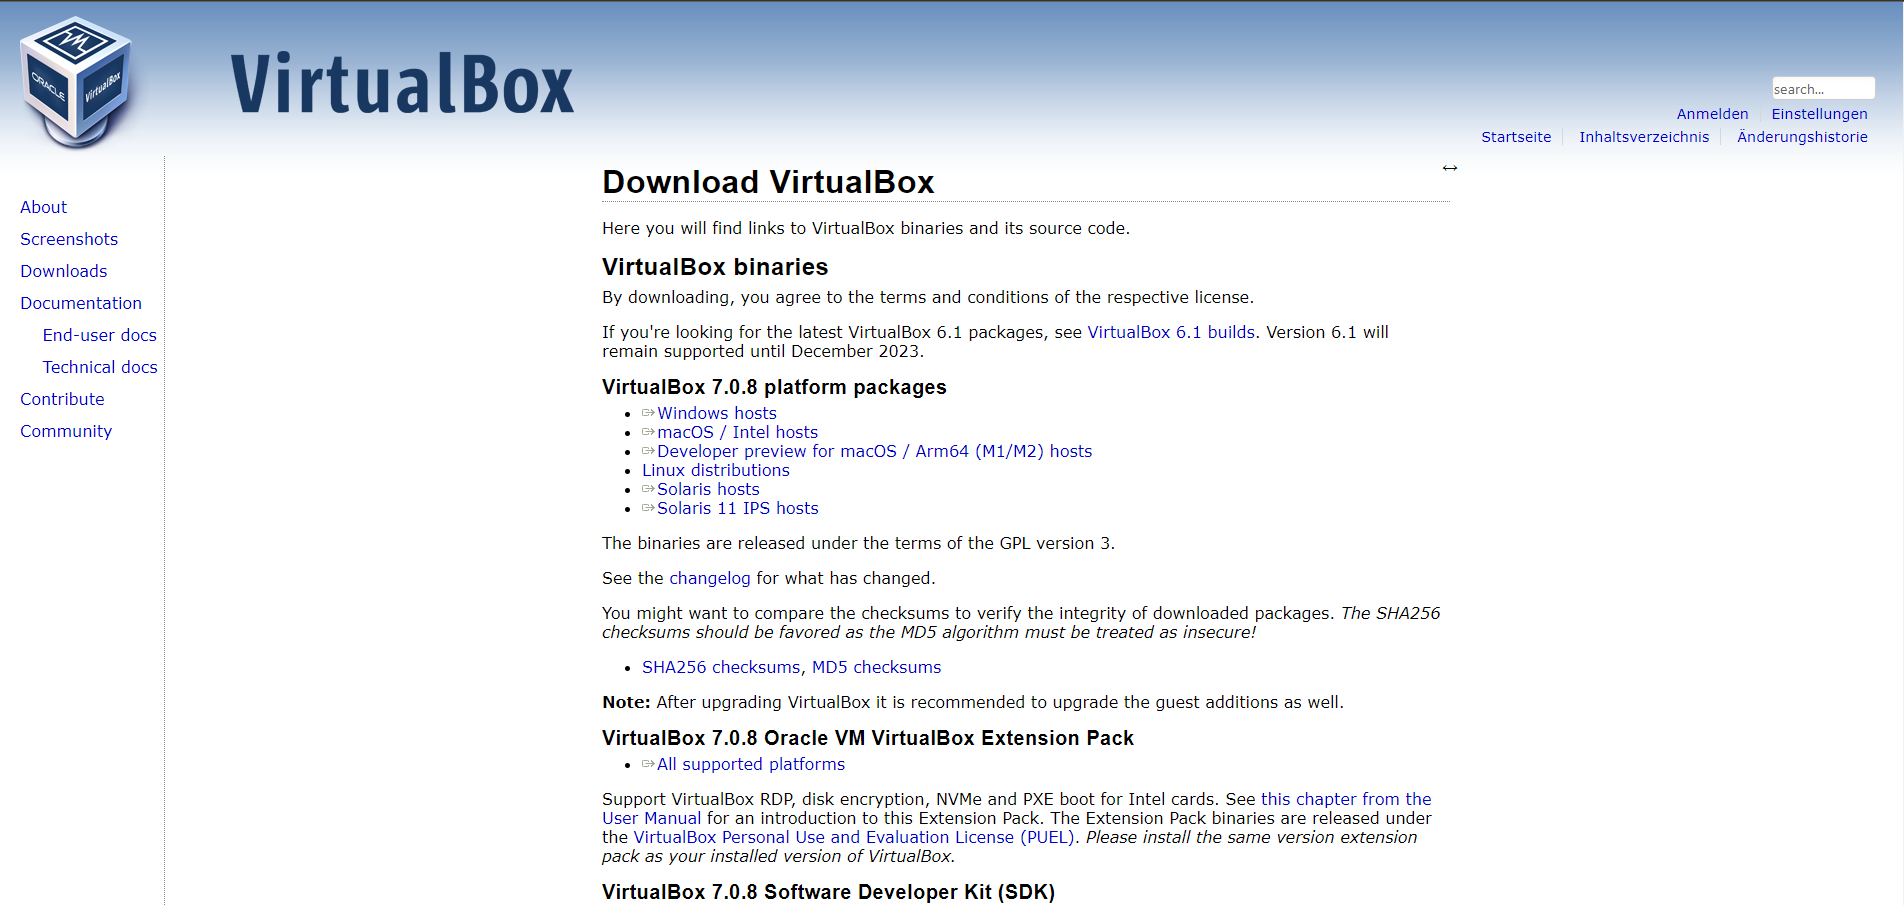
\includegraphics[width=\textwidth]{img/2./virtual_box_website.png}
\end{figure}

\noindent
On the website, you'll find various operating systems to choose from. Select the one that matches your device's system, and the download will begin automatically. To install it, open the downloaded file and follow the installation instructions.\\

\paragraph{Download Ubuntu 22.04 image}~\\
Next, you'll need to download the Ubuntu 22.04 LTS ISO image. Visit the official Ubuntu website \footnote{https://releases.ubuntu.com/jammy/} and download the image from there.

\begin{figure}[H]
    \centering
    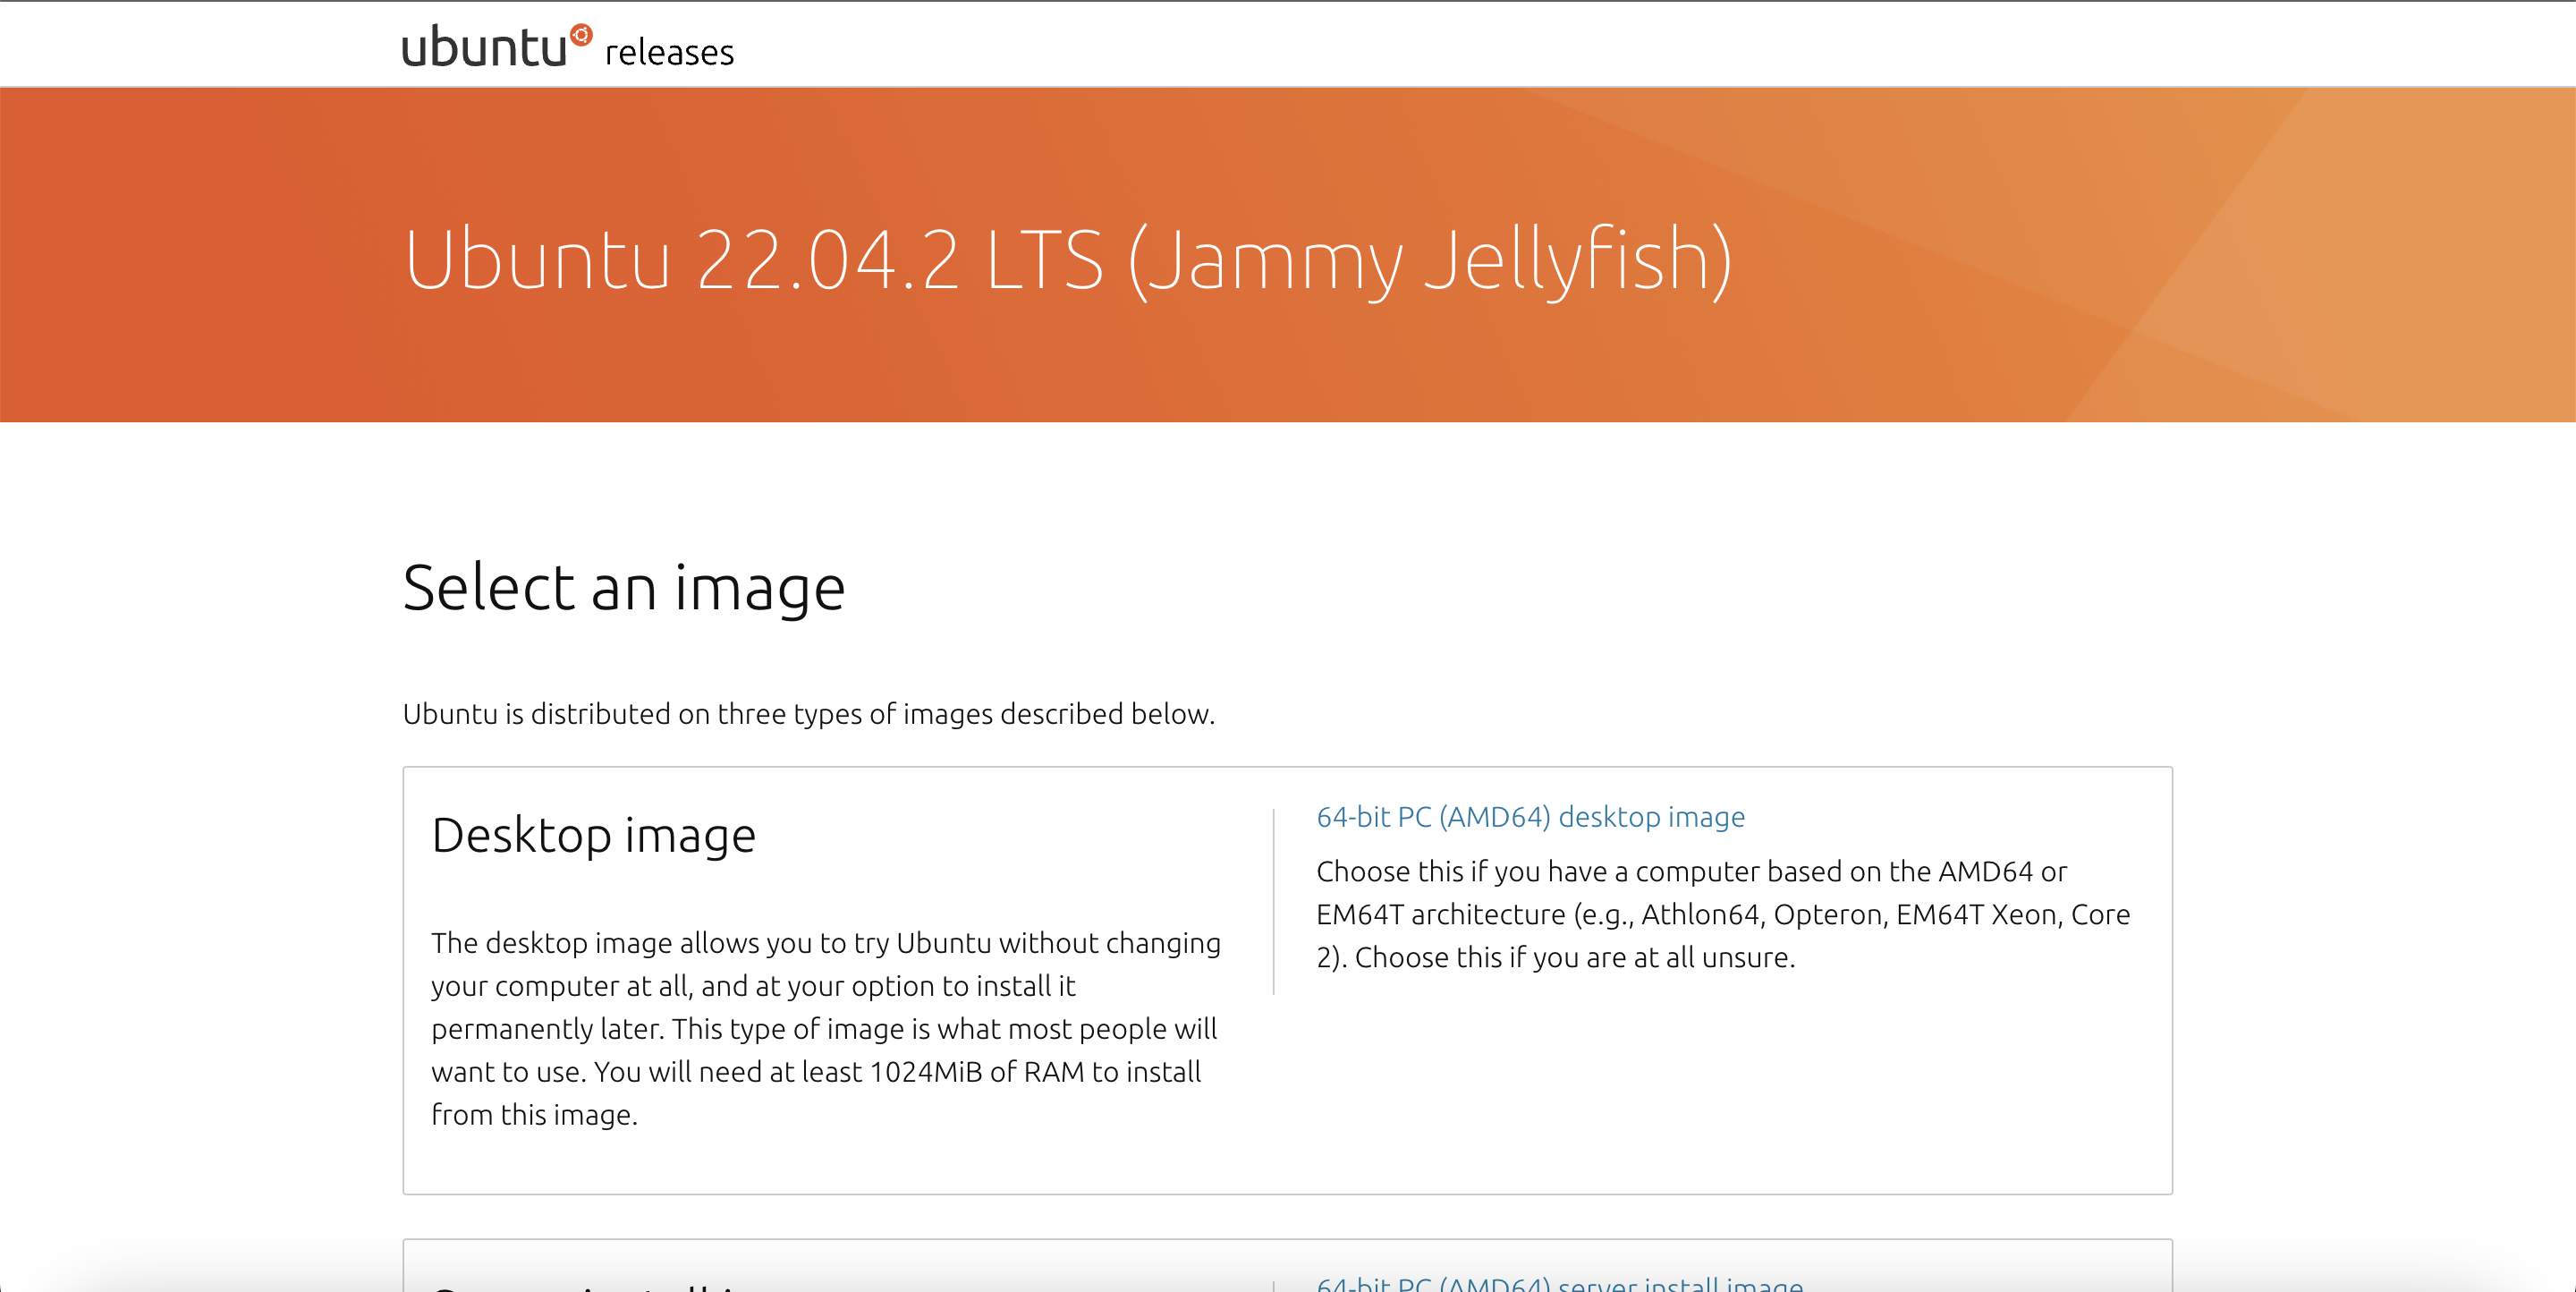
\includegraphics[width=\textwidth]{img/2./ubuntu_website.png}
\end{figure}

\paragraph{Create Virtual Machine}~\\
Since you've already installed VirtualBox, let's create a new virtual machine. When you launch VirtualBox, your screen should display the following image.

\begin{figure}[H]
    \centering
    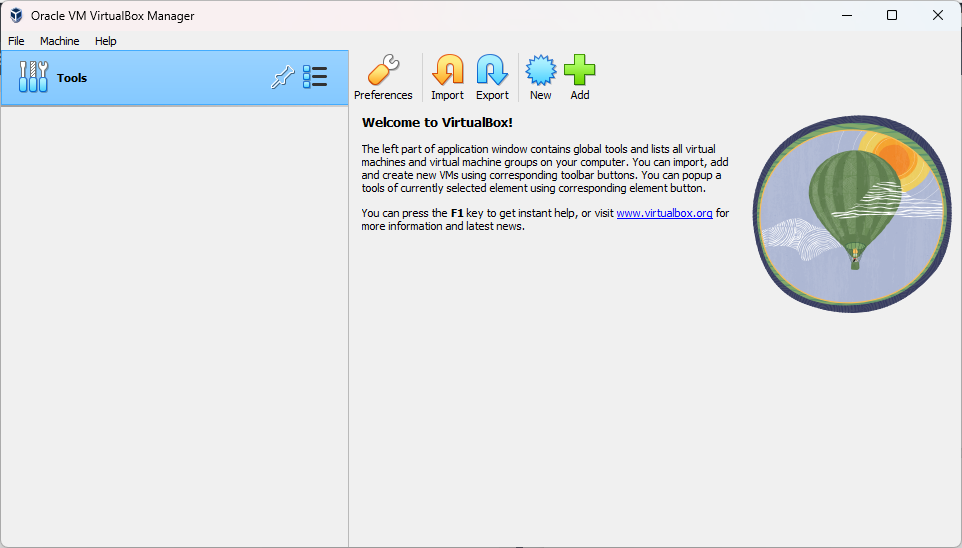
\includegraphics[width=\textwidth]{img/2./virtual_box1_english.png}
\end{figure}

\noindent
Click on the \textbf{New} button to initiate the creation of a new virtual machine. Provide a \textbf{Name} of your preference (e.g., Ubuntu 22.04), select the \textbf{Type} as Linux, and choose \textbf{Version} as Ubuntu (64-bit).

\begin{figure}[H]
    \centering
    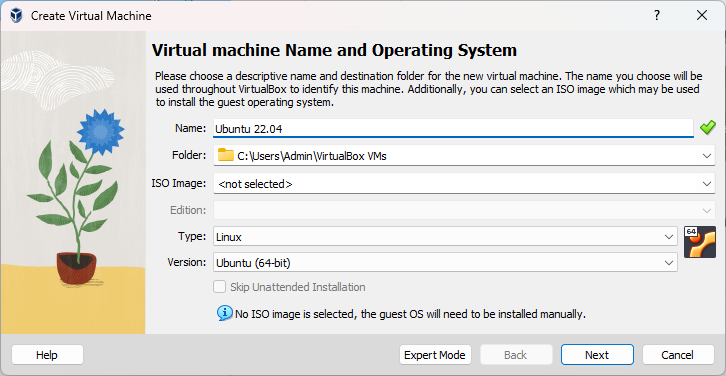
\includegraphics[width=\textwidth]{img/2./virtual_box2_english.png}
\end{figure}

\noindent
During the following step, proceed with the instructions to configure the amount of RAM and the number of CPUs allocated to your virtual machine. It is advisable to allocate a minimum of 2 GB of RAM. In our example, we'll allocate 8 GB from the device's total 16 GB of RAM and assign 3 CPUs. You can use the green bar as an orientation to make no mistakes.
        
\begin{figure}[H]
    \centering
    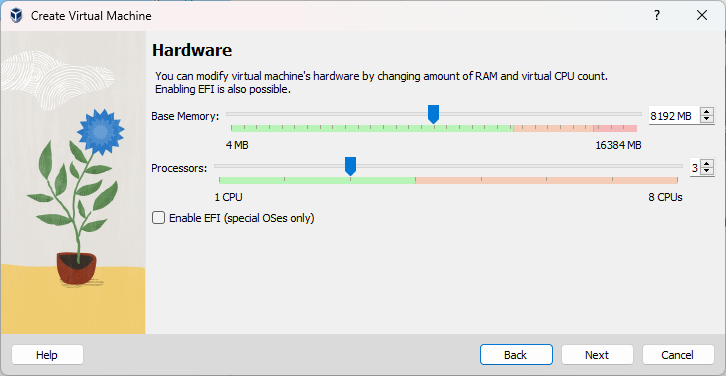
\includegraphics[width=\textwidth]{img/2./virtual_box3_english.png}
\end{figure}

\noindent
Next, you will need to create a new virtual hard disk or use an existing one if you have any. In our scenario, we allocate 30 GB of storage for the virtual hard disk. However, you should adjust the storage size based on the available space on your system.

\begin{figure}[H]
    \centering
    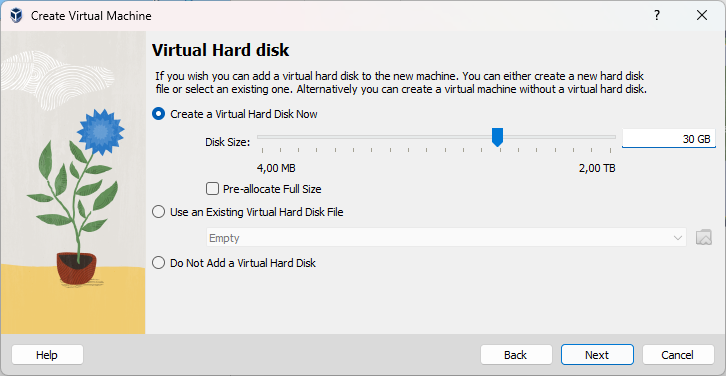
\includegraphics[width=\textwidth]{img/2./virtual_box4_english.png}
\end{figure}

\noindent       
Continue with the setup process, and your virtual machine should be almost ready for use. Your screen should resemble the following screenshot:

\begin{figure}[H]
    \centering
    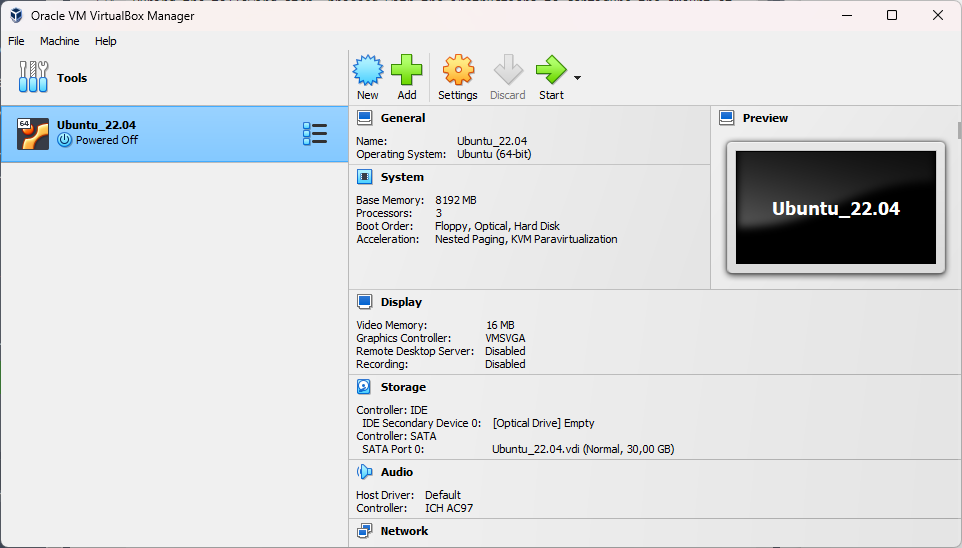
\includegraphics[width=\textwidth]{img/2./virtual_box5_english.png}
\end{figure}

\noindent
Inside the virtual machine settings, click on the “Storage” tab, then select the empty disk icon. Choose “Choose/Create a Disk” and navigate to the Ubuntu 22.04 ISO file you downloaded earlier. Select the ISO file and click “OK” to attach it to the virtual machine.

\begin{figure}[H]
    \centering
    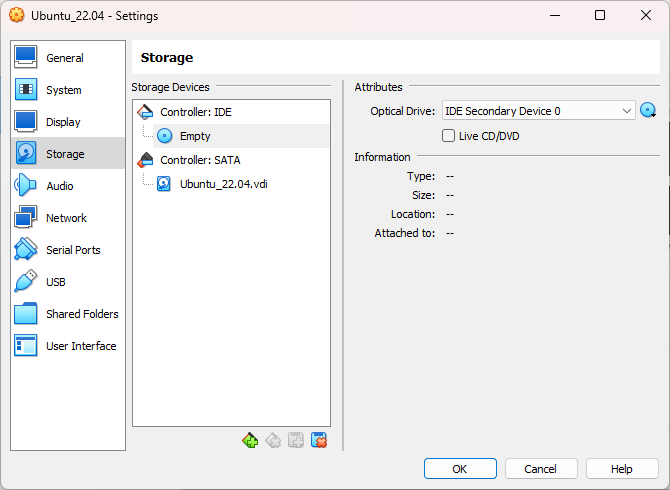
\includegraphics[width=\textwidth]{img/2./virtual_box6_english.png}
\end{figure}

\noindent
Now, to confirm whether you've set everything up correctly, select your virtual machine and start it by double-clicking on it.

\begin{figure}[H]
    \centering
    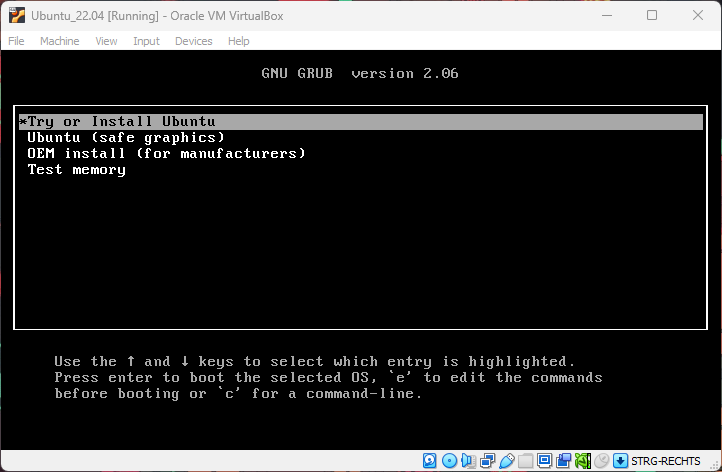
\includegraphics[width=\textwidth]{img/2./virtual_box7_english.png}
\end{figure}

\noindent
If it successfully starts up and you see the GRUB bootloader, congratulations! You have successfully set up your virtual machine. To proceed with installing Ubuntu, select the option “Try or Install Ubuntu” and follow the instructions provided in the installation setup.
        
\subsection{Install Ubuntu 22.04 with Dual Boot}
You seem to have chosen to install Ubuntu via dual boot. Installing Ubuntu in dual boot mode can be a bit more complex, so we recommend following a comprehensive installation guide. A good guide can be found at the freeCodeCamp website\footnote{https://www.freecodecamp.org/news/how-to-dual-boot-windows-10-and-ubuntu-linux-dual-booting-tutorial/}.\\
If you prefer visual instructions, you can search for “Ubuntu 22.04 dual boot installation” on YouTube.\\
\textit{Make sure to choose Ubuntu version 22.04, as this is the version recommended for working with ROS2 Humble.}

\newpage
\section{ROS2 Basics}
In this module, we will build a solid foundation in ROS2. We'll start by setting up ROS2 and dive into core concepts such as nodes, topics, and services. You'll gain the skills to create ROS2 workspaces and packages, setting the stage for you to work with real-world components. It's crucial to master these ROS2 fundamentals before going on with practical applications.

    
\subsection{Setting up ROS2}
If you have successfully installed Ubuntu on your device or within a virtual machine, you are now ready to proceed with the installation of ROS2. In the following sections, we will guide you through the process of installing ROS2 \footnote{https://foxglove.dev/blog/installing-ros2-humble-on-ubuntu}.

\paragraph{Set the Locale}~\\
Before installing ROS2, it's recommended to set the locale for your system to ensure proper language and formatting settings. You can choose the US locale to ensure everything works smoothly. Open a terminal and enter the following command to set the locale:

{\lstconsolestyle
\begin{lstlisting}
$ sudo apt update && sudo apt install locales
$ sudo locale-gen en_US en_US.UTF-8
$ sudo update-locale LC_ALL=en_US.UTF-8 LANG=en_US.UTF-8
$ export LANG=en_US.UTF-8       
\end{lstlisting}
}

\paragraph{Set up Your Source Repository}~\\
Ubuntu's software organization is structured into repositories, which ensures secure software installation. The main repositories in Ubuntu are categorized as follows:
\begin{enumerate}
    \item[$\bullet$]\texttt{Main} (canonical-supported open-source software)
    \item[$\bullet$]\texttt{Universe} (community-maintained open source software)
    \item[$\bullet$]\texttt{Restricted} (proprietary device drivers)
    \item[$\bullet$]\texttt{Multiverse} (proprietary software)
\end{enumerate}
For the purpose of installing ROS2, we have to make sure the Ubuntu Universe repository is enabled.

{\lstconsolestyle
\begin{lstlisting}
$ sudo apt install software-properties-common
$ sudo add-apt-repository universe
\end{lstlisting}
}

\noindent
Once the Ubuntu Universe repository is enabled, you can proceed to add the ROS 2 repository to your system. This involves authorizing the public GPG\footnote{https://gnupg.org/} key provided by ROS 2 and adding the repository to your sources list.

{\lstconsolestyle
\begin{lstlisting}
$ sudo apt update && sudo apt install curl gnupg lsb-release
$ sudo curl -sSL https://raw.githubusercontent.com/ros/rosdistro/master/ros.key -o /usr/share/keyrings/ros-archive-keyring.gpg
$ echo "deb [arch=$(dpkg --print-architecture) signed-by=/usr/share/keyrings/ros-archive-keyring.gpg] http://packages.ros.org/ros2/ubuntu $(source /etc/os-release && echo $UBUNTU_CODENAME) main" | sudo tee /etc/apt/sources.list.d/ros2.list > /dev/null
\end{lstlisting}
}

\paragraph{Install ROS2 packages} ~\\
There are three different ROS2 installation options to choose from:

\begin{enumerate}
    \item[$\bullet$] \texttt{Desktop Install}
    \item[$\bullet$] \texttt{ROS-Base Install}
    \item[$\bullet$] \texttt{Development tools}
\end{enumerate}

\noindent
It's important to note that each installation option installs a different set of packages. In our scenario, we've chosen the desktop installation because it comes with a comprehensive selection of packages, tools, libraries, and graphical interfaces. However, if you prefer to have more control over the installed packages, you can select the base installation and then add specific packages later according to your needs.

{\lstconsolestyle
\begin{lstlisting}
$ sudo apt update
$ sudo apt upgrade
$ sudo apt install ros-humble-desktop
\end{lstlisting}
}

\paragraph{Source your setup file} ~\\
Usually, you need to source the setup file in every new terminal to gain access to ROS2 commands.

{\lstconsolestyle
\begin{lstlisting}
$ source /opt/ros/humble/setup.bash
\end{lstlisting}
}

\noindent
We can save ourselves some work by adding this command to the .bashrc file. This bash shell script will be run whenever we open a new terminal.

{\lstconsolestyle
\begin{lstlisting}
$ echo "source /opt/ros/humble/setup.bash" >> ~/.bashrc
$ source ~/.bashrc
\end{lstlisting}
}

\paragraph{ROS2 Test}~\\
Next, let's continue by testing our ROS 2 environment using the following command:
    
{\lstconsolestyle
\begin{lstlisting}
$ ros2 run turtlesim turtlesim_node
\end{lstlisting}
}

\noindent
If this command opens a new window with a turtle inside, you successfully installed ROS2 Humble.\\
The window that opens is the turtlesim simulator, a tool we will use to learn the basics of ROS2 communication and how to control robots. Let's proceed with understanding the ROS2 communication system and how we can utilize it for controlling robots.

\subsection{ROS2 Communication}
\subsubsection{What is a Node}
In ROS2, each node\footnote{\label{fig:understanding_nodes}https://docs.ros.org/en/humble/Tutorials/Beginner-CLI-Tools/Understanding-ROS2-Nodes/Understanding-ROS2-Nodes.html\label{note1}} should be responsible for a single, modular purpose. All nodes work independently from each other and can only send and receive data from other nodes via topics, services, actions, or parameters (figure: \ref{figure:Communication}).


\begin{figure}[H]
    \centering
    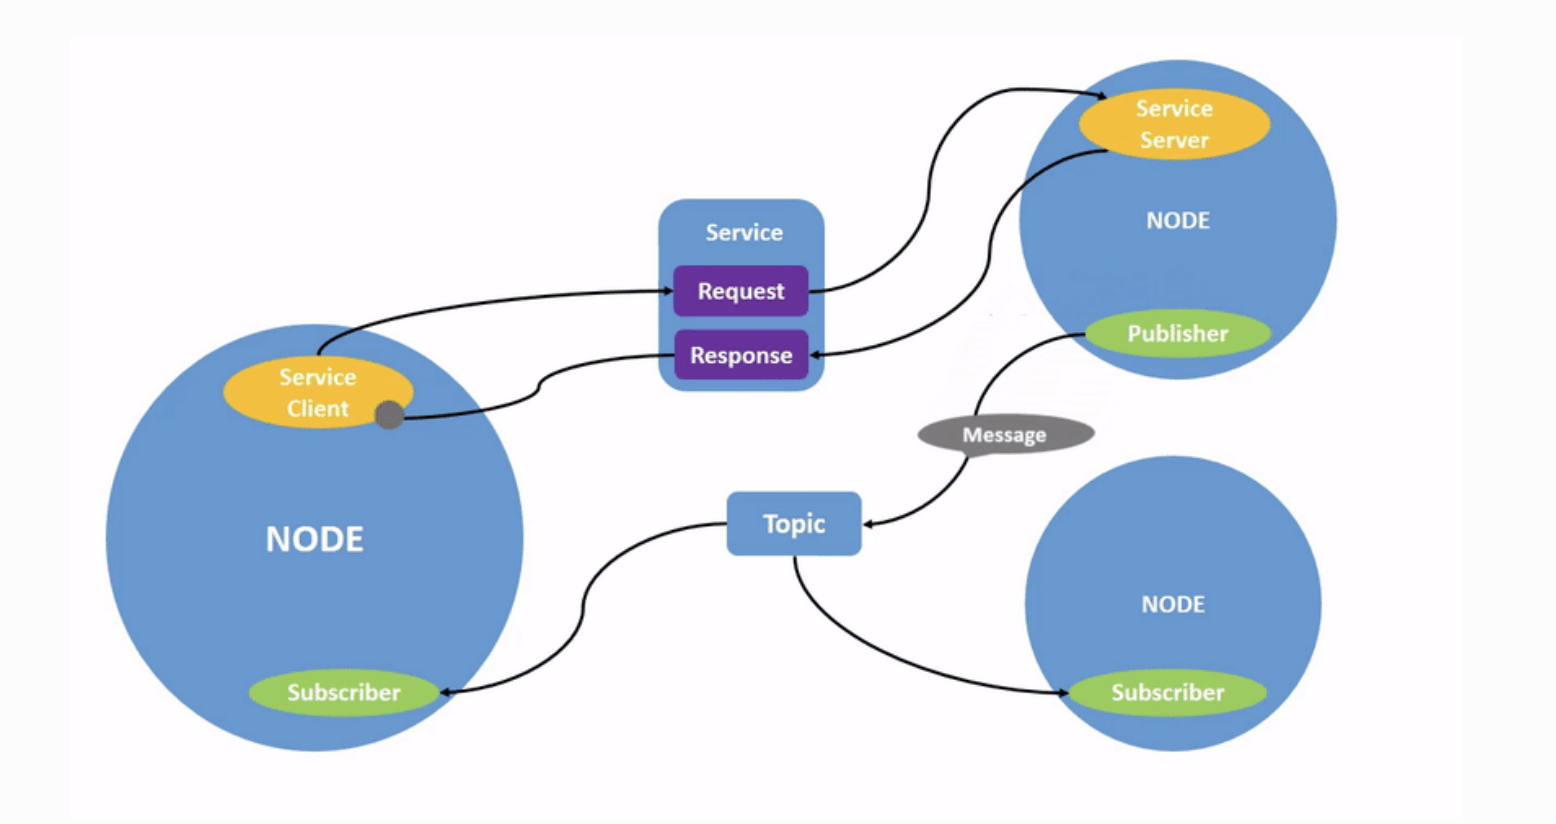
\includegraphics[width = \textwidth]{img/3.4/image.png}
    \caption[Communitcation Graph ROS2]{Communication Graph ROS2 \textsuperscript{\ref{fig:understanding_nodes}}}
    \label{figure:Communication}
\end{figure}

\subsubsection{Topics}
The most common way for nodes to communicate is with topics. Nodes can either subscribe to a topic or publish to it. When nodes publish to a topic, they send a message to it with a specific message type. Other nodes can then subscribe to the topic to receive these published messages. Nodes have no information about the other nodes, publishing or subscribing to a topic. Let's use a simple example to get a better idea of this concept.
\\


\paragraph{ros2 run}~\\
\noindent 
To run executables from a ROS2 package in your terminal, you can use the \texttt{ros2 run $<$package\_name$>$ $<$executable\_name$>$} command.
Let's try running the turtlesim\_node executable from the turtlesim package.

{\lstconsolestyle
\begin{lstlisting}
$ ros2 run turtlesim turtlesim_node
\end{lstlisting}
}

\noindent 
This command should look familiar. We already used it to check our ROS2 installation. It executes the turtlesim simulation. The executable turtlesim\_node creates a new node for the turtle that can be used to communicate with it.
\\
\paragraph{ros2 node list}~\\
The \texttt{ros2 node list} command will display a list of all currently active nodes. To execute this command, open a new terminal, as only one executable can run within a single terminal at a time.

{\lstconsolestyle
\begin{lstlisting}
$ ros2 node list
    /turtlesim
\end{lstlisting}}

\noindent
As you can observe, the command returns \texttt{/turtlesim}, which corresponds to the node that was generated by the \texttt{turtlesim\_node} script. To proceed, let's execute another script to create an additional node. (new terminal)

{\lstconsolestyle
\begin{lstlisting}
$ros2 run turtlesim turtle_teleop_key
\end{lstlisting}}

\noindent
The \texttt{turtle\_teleop\_key} is another executable provided by the \texttt{turtlesim} package. It enables you to control the turtle using your keyboard inputs. 
Now, if we list all nodes again, we can observe that a new node has been created with the name \texttt{/teleop\_turtle}.

{\lstconsolestyle
\begin{lstlisting}
$ ros2 node list
    /turtlesim
    /teleop_turtle
\end{lstlisting}}

\paragraph{ros2 node info}~\\
\noindent
We will now check out how the two nodes are able to communicate with each other.
To get further information on a node, you can use the command \texttt{ros2 node info $<$node\_name$>$}.
\noindent
The console returns an enumeration of all subscribers, publishers, services and actions that interact with the node. 

{\lstconsolestyle
\begin{lstlisting}
$ros2 node info /turtlesim
    Subscribers:
        /parameter_events: rcl_interfaces/msg/ParameterEvent
        /turtle1/cmd_vel: geometry_msgs/msg/Twist
    Publishers:
        /parameter_events: rcl_interfaces/msg/ParameterEvent
        /rosout: rcl_interfaces/msg/Log
        /turtle1/color_sensor: turtlesim/msg/Color
        /turtle1/pose: turtlesim/msg/Pose
    Service Servers:
        /clear: std_srvs/srv/Empty
        /kill: turtlesim/srv/Kill
        /reset: std_srvs/srv/Empty
        /spawn: turtlesim/srv/Spawn
        /turtle1/set_pen: turtlesim/srv/SetPen
        /turtle1/teleport_absolute: turtlesim/srv/TeleportAbsolute
        /turtle1/teleport_relative: turtlesim/srv/TeleportRelative
        /turtlesim/describe_parameters: rcl_interfaces/srv/DescribeParameters
        /turtlesim/get_parameter_types: rcl_interfaces/srv/GetParameterTypes
        /turtlesim/get_parameters: rcl_interfaces/srv/GetParameters
        /turtlesim/list_parameters: rcl_interfaces/srv/ListParameters
        /turtlesim/set_parameters: rcl_interfaces/srv/SetParameters
        /turtlesim/set_parameters_atomically:
        rcl_interfaces/srv/SetParametersAtomically
    Service Clients:
        
    Action Servers:
        /turtle1/rotate_absolute: turtlesim/action/RotateAbsolute
        Action Clients:   
\end{lstlisting}}

\noindent 
As you can observe, \texttt{/turtlesim} subscribes to the topic \texttt{/turtle1/cmd\_vel}. This topic communicates the linear and angular velocities of the turtle. Additionally, you can find details about the message type associated with this topic. You may notice that the topic \texttt{/turtle1/cmd\_vel} uses the \texttt{geometry\_msgs/msg/Twist} message type.\\

\noindent
If we repeat this step with /teleop\_turtle, we will observe that it publishes data to the same topic that /turtlesim subscribes to.
\paragraph{RQt}~\\
You have the option to get a graphical overview of all topics, their publishers, and subscribers using RQt. RQt is a graphical user interface framework that provides various tools and interfaces in the form of plugins.
To use RQt, you have to pen a new terminal and enter \texttt{rqt} to open the software.

{\lstconsolestyle
\begin{lstlisting}
$ rqt
\end{lstlisting}
}
\noindent
Inside RQt, select \texttt{Plugins $>$ Introspection $>$ Node Graph} to open the node graph. The node graph visualizes all nodes and topics that are currently running. If a node subscribes to a topic, an arrow points from the topic to the node, and if a node publishes data, the arrow points in the opposite direction. You can see an example of a node graph in figure \ref{figure:node graph}. It illustrates the communication of the nodes /turtlesim and /teleop\_turtle.
\begin{figure}[H]
    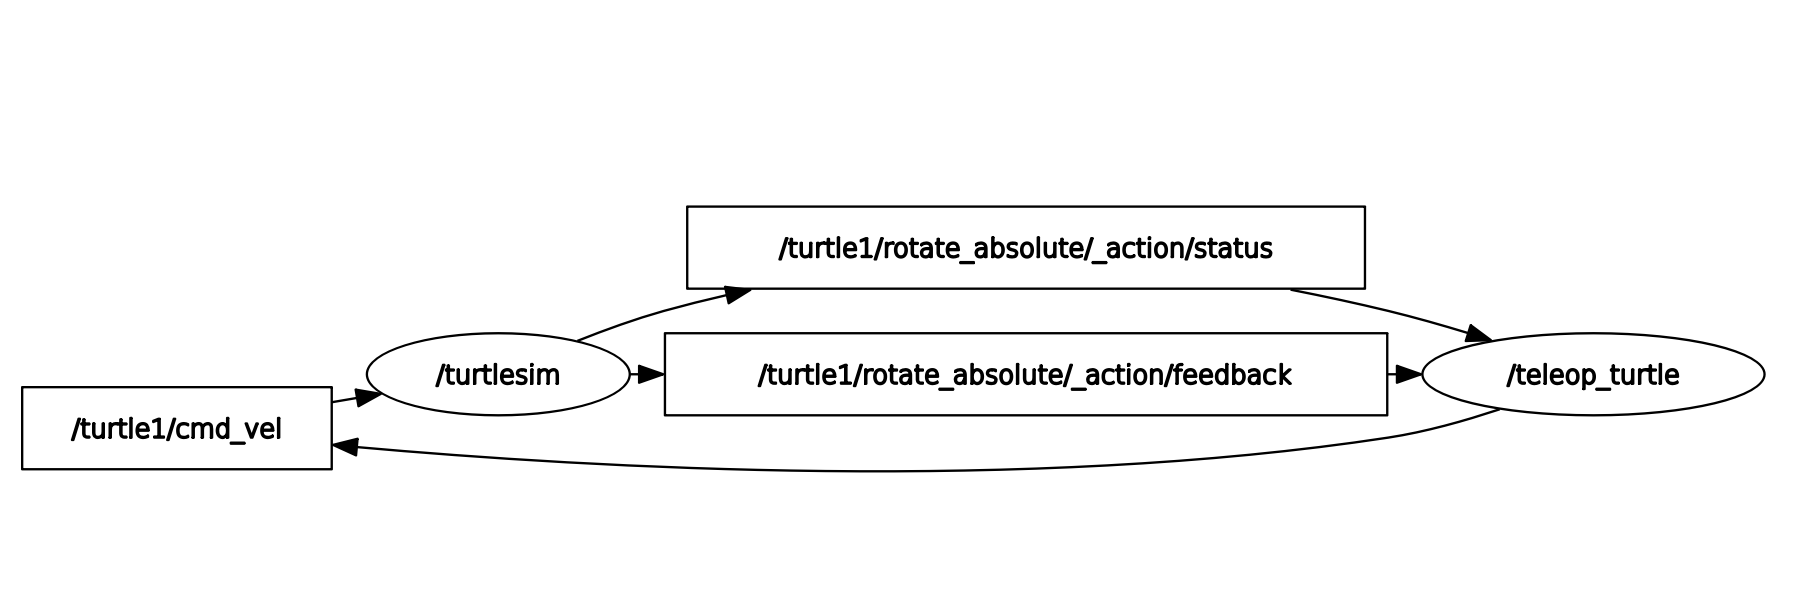
\includegraphics[width=  \textwidth]{img/Ros2Basics/Node_Graph.png}
    \caption{Node Graph Turtlesim}
    \label{figure:node graph}
\end{figure}

\noindent 
In contrast to the \texttt{ros2 node info} command, which only provides information on one node, this method allows us to get a picture of all nodes and topics. \\
One advantage of \texttt{ros2 node info} is the fact that you are able to see the message types of a topic the node is connected with.\\
But a more convenient way to do this is by using the command \texttt{ros2 topic info $<$topic\_name$>$}. \\
We will now check the \texttt{/turtle1/cmd\_vel} topic with this command. Remember, this is the topic \texttt{/turtlesim }subscribes to.
{\lstconsolestyle
\begin{lstlisting}
$ros2 topic info /turtle1/cmd_vel
    Type: geometry_msgs/msg/Twist
    Publisher count: 0
    Subscription count: 1
\end{lstlisting}}
\noindent 
As you can see, we get the same message type as before and, on top of that, the number of publishers and subscribers of our topic.\\

\paragraph{ros2 interface show}~\\
Now, let's explore how message types are defined and learn how to send our own messages.\\
With the help of the \texttt{ros2 interface show $<$package\_name$>$/$<$message\_type$>$} command, there is a straightforward method to inspect how different message types are defined.\\
When using the \texttt{geometry\_msgs/msg/Twist} message type, this command returns the following information.
{\lstconsolestyle
\begin{lstlisting}
$ros2 interface show geometry_msgs/msg/Twist
# This expresses velocity in free space broken into its linear and angular parts.

Vector3  linear
	float64 x
	float64 y
	float64 z
Vector3  angular
	float64 x
	float64 y
	float64 z

\end{lstlisting}}
\noindent As you can observe, each message contains two vectors that describe a linear and an angular velocity. When a message with this message type is published to the \texttt{/turtle1/cmd\_vel} topic, the \texttt{/turtlesim} node utilizes this message to control the turtle's movement.\\

\paragraph{ros2 topic echo}~\\
We will now make use of the \texttt{teleop\_turtle} node to observe the contents of the messages generated by pressing the arrow keys. The command \texttt{ros2 topic echo $<$topic\_name$>$} can be employed to display all the messages that are published to a specific topic. Whenever a message is published to that topic, this command will display the message in the terminal.

{\lstconsolestyle
\begin{lstlisting}
$ ros2 topic echo /turtle1/cmd_vel
\end{lstlisting}}

\noindent
To send a single message, we press the \texttt{UP\_Arrow} key on our keyboard within the \texttt{teleop\_turtle} terminal. In the \texttt{turtlesim} window, you'll notice that the turtle moves straight forward for a brief moment. To inspect the content of the message, we can observe the output in our \texttt{ros2 topic echo} terminal. You might notice that it displayed the message content as soon as we pressed the key.

{\lstconsolestyle
\begin{lstlisting}
$ ros2 topic echo /turtle1/cmd_vel 
    linear:
      x: 2.0
      y: 0.0
      z: 0.0
    angular:
      x: 0.0
      y: 0.0
      z: 0.0
    ---
\end{lstlisting}}

\noindent
It is logical that the message only contained a linear x value, given that the turtle moved straight forward.

\paragraph{exercise}~\\
\begin{enumerate}
    \item[1.)] Use all arrow keys to move the turtle around. How does the turtle react to the different keys?
    \item[2.)] Take a look at the messages that are sent for all different arrow keys.
    \item[3.)] Why are there just two different values of geometry\_msgs/msg/Twist relevant for this simulation?
\end{enumerate}


\subsubsection{Publish a Message}
\paragraph{ros2 topic pub}~\\
Our next objective is to publish a custom message to the /turtle1/cmd\_vel topic. To achieve this, you'll use the command \texttt{ros2 topic pub -r $<$rate$>$ $<$topic\_name$>$ $<$message\_type$>$ $<$message\_options$>$} in your terminal. The rate, specified in Hz, determines how frequently your message will be published. Because the turtlesim plane is limited to a two-dimensional space and the turtle is restricted to move in the x direction, it is only necessary to publish the linear x data and angular z data. For the syntax of the published message, use curly brackets within quotation marks, following this format (YAML syntax): \texttt{\{\{ \text{linear:} \{x: 1\}, \text{angular:} \{z: 1\}\}\}}\\

\noindent
Now, let's publish a message with a linear x value of 1 and an angular z value of 1 every second to achieve circular motion of the turtle.
{\lstconsolestyle
\begin{lstlisting}
$ ros2 topic pub -r 1 /turtle1/cmd_vel geometry_msgs/msg/Twist "{linear: {x: 2}, angular: {z: 1}}"
\end{lstlisting}}

\noindent 
If done correctly, the turtle should now continuously move in a circle.\\
To end the task, use the keyboard shortcut \texttt{CTRL + C}. \\

\paragraph{exercise}~\\
\begin{enumerate}
    \item[$\bullet$] Test different values for x and z. What happens if you just publish a linear or an angular value?
    \item[$\bullet$] In another terminal, use the ros2 topic echo command and take a look at the messages.
    \item[$\bullet$] Use the flag -1 for the ros2 topic pub command. What is the effect of using it?
\end{enumerate}

\paragraph{RQt Message Publisher}~\\
A more straightforward method to publish messages is by using RQt. Open the program and go to \texttt{Plugins $>$ Topics $>$ Message Publisher} to select the message publisher plugin. To refresh all topics, click on the two blue arrows in the upper left corner. Now, choose the topic /turtle1/cmd\_vel to specify where you want to send your message. The Message Publisher will automatically recognize the correct message type, which is geometry\_msgs/msg/Twist. You can optionally adjust the frequency, but for this task, 1 Hz is sufficient. Click the blue plus button to add your chosen topic. It should now be listed in your publisher.
To send the same message as before, enter 1.0 in the expression cell of linear: x and angular: z. Then, select the box on the left of your topic to activate it. This step should produce the same outcome as when using the \texttt{ros2 topic pub} command.

\begin{figure}[H]
    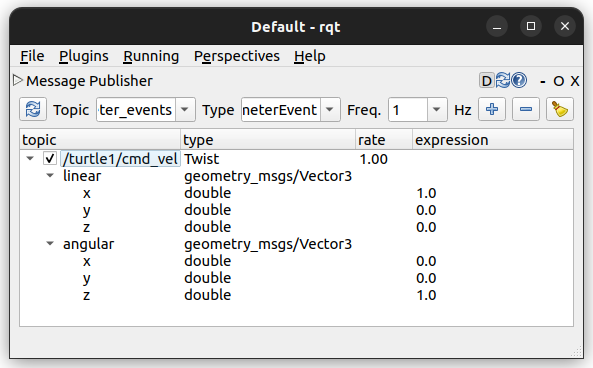
\includegraphics[width=  \textwidth]{img/Ros2Basics/RQt_message_publisher.png}
    \caption{RQt Message Publisher}
    \label{figure:message_publisher}
\end{figure}

\subsection{Setup ROS2 Workspace} 
Our next objective is to create our own publisher and subscriber nodes. However, before we can begin writing code, we need to create a workspace that will contain all the packages that we are going to create. Each package generally serves a specific purpose.\\
ROS2 provides various systems for building packages. The most common options include ament\_python and ament\_cmake. Throughout this course, we will primarily utilize ament\_python for our packages, given our focus on Python programming. The alternate approach to writing ROS2-specific code involves using C++, which would require using CMake to build the package. The main advantage of using Python is its simplicity and ease of use, making it an excellent choice for beginners. On the other hand, C++ excels in terms of performance. Since this is a beginner's course, we are going to use Python and, therefore, ament\_python to build our packages.

\paragraph{Colcon}\footnote{https://docs.ros.org/en/foxy/Tutorials/Beginner-Client-Libraries/Colcon-Tutorial.html}~\\
First and foremost, before we can proceed with building a package, we need to ensure that colcon is installed. Colcon serves as the tool for building and managing packages within ROS2.
    
{\lstconsolestyle
\begin{lstlisting}
$ sudo apt install python3-colcon-common-extensions
\end{lstlisting}
}

\noindent
Our next task is to build our workspace. A ROS2 workspace is a directory with a specific structure. It usually includes a 'src' subdirectory, which is where our packages are stored.

\begin{figure}[H]
    \centering
    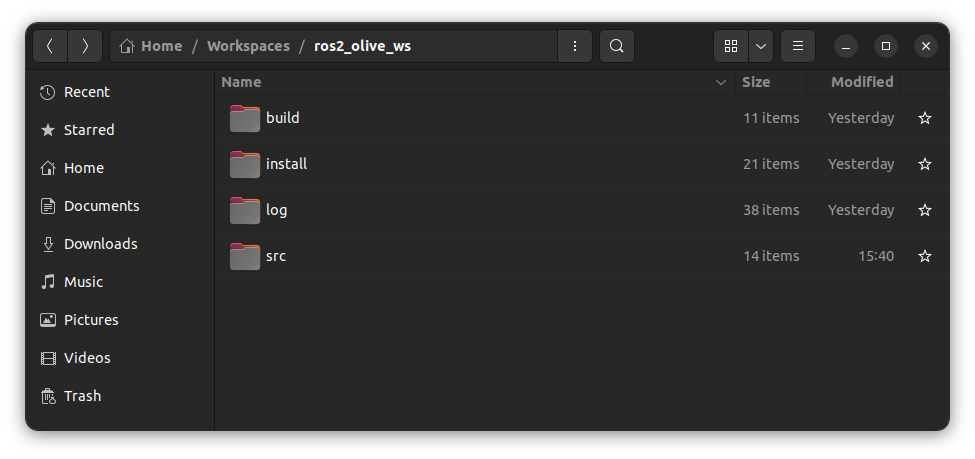
\includegraphics[width=  \textwidth]{img/workspace/workspace.png}
    \caption{Structure of a ROS2 workspace}
\end{figure}

\noindent
For now, let's focus on the src directory. We need to be able to navigate inside our terminal to be able to continue our task. In Linux, the standard method for navigation in the terminal is using the \texttt{cd <directory>} (Change Directory) command. To move to the \texttt{\$HOME} directory, you can utilize \texttt{cd $\sim$}. Another significant Linux command is \texttt{ls} (List), which provides an overview of all items in your present directory. Tab completion is often beneficial for command autocompletion.
{\lstconsolestyle
\begin{lstlisting}
$ cd ~
$ ls
Desktop    Downloads  Pictures  snap       Videos
Documents  Music      Public    Templates
\end{lstlisting}
}

\noindent
This structure is how our \texttt{\$HOME} directory should look like. We frequently use \\ \texttt{$\sim$/directory/directory/...} to create paths, starting from our \texttt{\$HOME} directory. Within your home directory, establish a new directory for all your workspaces. To generate a new directory, use the \texttt{mkdir} command succeeded by the desired folder name. Afterwards, navigate into the folder using the \texttt{cd} command.
{\lstconsolestyle
\begin{lstlisting}
$ mkdir Workspaces
$ ls
Desktop    Downloads  Pictures  snap       Videos
Documents  Music      Public    Templates  Workspaces
$ cd Workspaces
\end{lstlisting}
}

\noindent
We will now proceed to create a new directory named \texttt{ros2\_olive\_ws}. This directory will serve as a storage of all the ROS2-specific content we are going to develop throughout this course.
{\lstconsolestyle
\begin{lstlisting}
$ cd Workspaces
$ mkdir ros2_olive_ws
$ cd ros2_olive_ws
\end{lstlisting}
}

\paragraph{colcon build}~\\
Execute the \texttt{colcon build} command within the root of your workspace to initiate the build process. After running this command, if you list the contents of your workspace, you will observe the addition of three new folders: \texttt{build}, \texttt{install}, and \texttt{log}. However, you might notice that the \texttt{src} folder has not been created automatically. This is why it's necessary for us to create it manually.
{\lstconsolestyle
\begin{lstlisting}
$ colcon build
$ ls
build  install log
$ mkdir src
$ ls
build  install  log  src
\end{lstlisting}
}
    
\noindent
Now that you've set up your workspace, you're all set to start making your first package.
    

\subsection[Creating a Package]{Creating a Package\footnote{https://docs.ros.org/en/foxy/Tutorials/Beginner-Client-Libraries/Creating-Your-First-ROS2-Package.html}}
Before we move on to creating our first package, let's take a moment to understand what a package actually is. In simple terms, it's a structured folder that contains code, configuration files, and resources dedicated to a particular function or component of a robot system.
\paragraph{ros2 pkg list}~\\
ROS2 already has a lot of packages included. Just to get a small overview of how many packages are already installed,  use the \texttt{ros2 pkg list} command.
You have already been using a package in previous examples. If you scroll through the list, you can see that turtlesim is a package that is already part of ROS2.
{\lstconsolestyle
\begin{lstlisting}
$ ros2 pkg list
(...)
topic_monitor
tracetools
trajectory_msgs
turtlesim
uncrustify_vendor
unique_identifier_msgs
(...)
\end{lstlisting}
}

\noindent
However, we are interested in creating our own package to be able to code custom software for our specific use.

\paragraph{ros2 pkg create}~\\
Before we can create a package, we always have to make sure to be in the right directory (src). To create a package in ROS2, use the command \texttt{ros2 pkg create $<$pkg\_name$>$}. Since we chose to use the tool ament\_python to build our packages, we have to add \texttt{--build-type ament\_python} to our command. Without using this option, the command automatically creates a CMake package by default.

{\lstconsolestyle
\begin{lstlisting}
$ ros2 pkg create test_package --build-type ament_python
$ cd test_package
$ ls
package.xml  resource  setup.cfg  setup.py  test  test_package
\end{lstlisting}
}

\noindent
After creating our package, it is noticeable that inside the new package folder, different new elements have been created.
\begin{enumerate}

\item[$\bullet$] \texttt{package.xml} contains metadata about the package, including its name, version, description, dependencies, and more.

\item[$\bullet$] \texttt{resource} can be used to store non-Python resources such as configuration files, data files, images, etc.

\item[$\bullet$] \texttt{setup.cfg} and \texttt{setup.py} are used by the Python setuptools package to define the package's metadata and installation information.

\item[$\bullet$] \texttt{$<$package\_name$>$} is the main Python folder that contains all of the Python code of our package.
\end{enumerate}

\subsection[Creating our first Nodes]{Creating our first Nodes\footnote{https://docs.ros.org/en/foxy/Tutorials/Beginner-Client-Libraries/Writing-A-Simple-Py-Publisher-And-Subscriber.html}}

 We finally set up everything to be able to write our first Python scripts. In this first small example, we will create two separate Python scripts. First, we are going to create a script, generating a node that publishes a random number to a topic. The other script will create a node that subscribes to the same topic and prints the received messages to the console.


\subsubsection{Structure of a Publisher Node in Python}
\noindent
Before we start to write the code for our publisher, let's take a look at the common structure of a publisher and subscriber in Python. 

\begin{minted}{python}
import rclpy
from rclpy.node import Node     # Import the node class
from std_msgs.msg import Int32  # Import the message type
\end{minted}

\noindent
At the beginning of our code, we have to import all necessary modules from \texttt{rclpy} and message types. The node class type will be used to create every custom node class. In this example, \texttt{Int32} has to be imported since it will be used as a message type for the topic. You can get further information about different message types in the official ROS2 docs \footnote{https://docs.ros.org/en/foxy/Concepts/About-ROS-Interfaces.html}.

    
\begin{minted}{python}
class MyPublisher(Node):
    def __init__(self):
        super().__init__('my_publisher')  # Specify node name
        # Create publisher
        self.publisher_ = self.create_publisher(Int32, 'my_topic', 10) 
        # Create a timer
        self.timer = self.create_timer(1.0, self.callback_funtion)  
\end{minted}

\begin{enumerate}

\item[$\bullet$] In the next step, we have to define our publisher node. By adding \texttt{Node} to the bracket of our class, we inherit the rclpy node class we imported.

\item[$\bullet$] In the constructor of our new class, we call the \texttt{\_\_init\_\_} function of the parent class using \texttt{super().\_\_init\_\_('my\_publisher')}. This call sets the name of the created node to 'my\_publisher'.

\item[$\bullet$] To create a publisher, we call the \texttt{create\_publisher(MessageType, topic\_name, qos\_profile)} function. In this case, we set MessageType to Int32, the topic\_name to 'my\_topic' and the qos\_profile to 10. A qos\_profile of 10 creates a queue with the queue\_size of 10. The queue\_size(depth) is a QoS(Quality of Service) setting that creates a buffer to counter problems like subscriber lag.

\item[$\bullet$]To publish messages, we have to create a timer. To do this, we use the \texttt{create\_timer}(interval, callback\_function) function. It calls the callback\_function in a specified interval that is defined in seconds.
\end{enumerate}

\begin{minted}{python}
        def callback_function(self):
        msg = Int32()  # Create an instance of the message type
        msg.data = 7  # Set the message data
        self.publisher_.publish(msg)  # Publish the message
        self.get_logger().info('Published: %d' % msg.data) 
    \end{minted}

    \begin{enumerate}
        \item[$\bullet$] We define the callback\_function as a function of our node class. It is called by the timer and will be used to publish our messages.
        \item[$\bullet$] Before we can publish a message, we have to create an instance of the message type we want to publish.\\
        \textit{Remember that you can inspect the structure of interfaces using ros2 interface show interface\_name}.
        {\lstconsolestyle
        \begin{lstlisting}
$ ros2 interface show std_msgs/msg/Int32
# This was originally provided as an example message.
# It is deprecated as of Foxy
# It is recommended to create your own semantically meaningful message.
# However if you would like to continue using this please use the equivalent in example_msgs.

int32 data

\end{lstlisting}}
As you can see, the Int32 interface only has an integer data input. We set the data value of our message to a value of our choice. 
\item[$\bullet$] Since we set up the message, we are now able to publish it using the \texttt{publish(message)} method, which is part of the publisher we created. The message will then be published to the topic of this publisher('my\_topic').
\item[$\bullet$] A step that is optional but useful is to print the data to the terminal. We use the \texttt{get\_logger().info('...')} method for this task, which is part of the node class. This will be useful to get feedback on the published data.
\end{enumerate}
    
\begin{minted}{python}  
def main(args=None):
    rclpy.init(args=args)
    publisher = MyPublisher()  # Create an instance of the publisher node class
    rclpy.spin(publisher)  # Spin the node
    publisher.destroy_node()  # Clean up
    rclpy.shutdown()

if __name__ == '__main__':
    main()
\end{minted}

\begin{enumerate}
\item[$\bullet$] \texttt{rclpy.init}(args) is used to initialize the ROS2 communication system. It is important to call it at the beginning of our main function.

\item[$\bullet$] In the next step, we have to create an instance of the custom node class.

\item[$\bullet$] \texttt{rclpy.spin()} starts the event loop. It is responsible for managing the callbacks of various callbacks \footnote{https://docs.ros2.org/latest/api/rclpy/api/init\_shutdown.html}. It's important to note that rclpy.spin() is a blocking call. The script will stay in the event loop until the node is shut down using the \texttt{node.destroy\_node()} call or an external signal.

\item[$\bullet$] With \texttt{rclpy.shutdown()}, we shut down previously used resources of ROS2 like nodes etc.
\end{enumerate}

\subsubsection{Structure of a Subscriber in Python}
\begin{minted}{python}
import rclpy
from rclpy.node import Node
from std_msgs.msg import Int32  # Import the message type

class MySubscriber(Node):
    def __init__(self):
        super().__init__('my_subscriber')  # Specify node name
        self.subscription = self.create_subscription(
            Int32,
            'my_topic',
            self.callback,
            10
        )

    def callback(self, msg):
        self.get_logger().info(f'Received: {msg.data}')

def main(args=None):
    rclpy.init(args=args)
    subscriber = MySubscriber()  # Create an instance of the subscriber node class
    rclpy.spin(subscriber)  # Spin the node
    subscriber.destroy_node()  # Clean up
    rclpy.shutdown()

if __name__ == '__main__':
    main()
\end{minted}

\noindent
The code to create a subscriber node looks quite similar to the publisher, but there are some key differences.
    
\begin{enumerate}
\item[$\bullet$] Instead of a publisher, you obviously create a subscription using 
 the \\ \texttt{create\_subscription(MessageType, topic\_name, callback, qos\_profile)} method. You don't need a timer to call the callback function. Instead, it is called whenever a message is received.
 
\item[$\bullet$] The callback function has two inputs, \texttt{self}(the node) and the message that is received.
\end{enumerate}

\noindent
Since we are now aware of how we can create our own nodes, we can go on with using this information to create a random number publisher and subscriber.

\subsubsection{Random number Publisher Script}
We are going to create a new package inside the src folder of our workspace for this task. We will call our new package \texttt{random\_number\_ps}. After creating the package, we navigate to the \texttt{random\_number\_ps} folder inside the package. In our script folder, we create a new Python script with the name \texttt{random\_number\_publisher.py} by using the VS Code command \texttt{code}. This command only works if  Visual Studio Code is installed and is used to edit or create a file in VS Code.

{\lstconsolestyle
\begin{lstlisting}
$ cd ~/Workspaces/ros2_olive_ws/src/
$ ros2 pkg create random_number_ps --build-type ament_python
$ cd random_number_ps
$ ls
package.xml  random_number_ps  resource  setup.cfg  setup.py  test
$ cd random_number_ps
$ code random_number_publisher.py
\end{lstlisting}
}

\begin{minted}{python}
import rclpy
from rclpy.node import Node
from std_msgs.msg import Int32
import random
\end{minted}

\noindent
The header of our random number publisher looks almost identical to before. We will publish a message of the \texttt{Int32} message type. The random module has to be imported to create the random number we want to publish.

\begin{minted}{python}
class RandomNumberPublisher(Node):
    def __init__(self):
        super().__init__('random_number_publisher')
        self.publisher_ = self.create_publisher(Int32, 'random_numbers', 10)
        self.timer = self.create_timer(1.0, self.publish_random_number)

    def publish_random_number(self):
        random_number = random.randint(1, 100)
        self.get_logger().info(f'Publishing: {random_number}')
        msg = Int32()
        msg.data = random_number
        self.publisher_.publish(msg)
\end{minted}

\noindent
This structure is the node class setup of our RandomNumberPublisher node. It initializes a node with the name \texttt{random\_number\_publisher}, which is used to call the \texttt{publish\_random\_number} function every second. \texttt{random.randint(1, 100)} is used to create a random number between 1 and 100. You can get further information about the random library in the python docs \footnote{https://docs.python.org/3/library/random.html}. We publish it to the topic \texttt{random\_numbers} and print it to the console with \texttt{get\_logger().info}.

\begin{minted}{python}
def main(args=None):
    rclpy.init(args=args)
    random_number_publisher = RandomNumberPublisher()
    rclpy.spin(random_number_publisher)
    random_number_publisher.destroy_node()
    rclpy.shutdown()

if __name__ == '__main__':
    main()
\end{minted}

\noindent
The last part is just as in the previous subscriber example.\\

\paragraph{declare dependencies}~\\
Before we can go on running our code, there are some steps we have to take to be able to build our package. \\
\noindent
One of those things is to declare the dependencies of our package. You do this inside the \texttt{package.xml} file of the package folder.\\
    
{\lstconsolestyle
\begin{lstlisting}
$ cd ~/Workspaces/ros2_olive_ws/src/random_number_ps/
$ ls
package.xml  random_number_ps  resource  setup.cfg  setup.py  test
$ code package.xml
\end{lstlisting}}

    \noindent
    
\begin{lstlisting}[caption={\texttt{package.xml file}}, captionpos=b]   
<?xml version="1.0"?>
<?xml-model href="http://download.ros.org/schema/package_format3.xsd" 
schematypens="http://www.w3.org/2001/XMLSchema"?>
<package format="3">
  <name>random_number_ps</name>
  <version>0.0.0</version>
  <description>TODO: Package description</description>
  <maintainer email="fabian@todo.todo">fabian</maintainer>
  <license>TODO: License declaration</license>

  <test_depend>ament_copyright</test_depend>
  <test_depend>ament_flake8</test_depend>
  <test_depend>ament_pep257</test_depend>
  <test_depend>python3-pytest</test_depend>

  <export>
    <build_type>ament_python</build_type>
  </export>
</package>
\end{lstlisting}

\noindent
Inside the package.xml file, we can change package information like the version, the description, etc. But for now, we just want to add the following lines after the ament\_python buildtool dependency. By declaring these runtime dependencies in the package.xml file, we are informing ROS2 about the packages that the package relies on to function correctly. 

\begin{lstlisting}
<exec_depend>rclpy</exec_depend>
<exec_depend>std_msgs</exec_depend>
\end{lstlisting}
    
\paragraph{Adding an entry point}~\\
Before we can run our script in the terminal with the ros2 run command, it is essential to edit the \texttt{setup.py} file inside the package folder. We have to add an entry point to the script.
For this task, open your setup.py file in VS Code. The content of the file should look like this:

\begin{minted}{python}
from setuptools import setup

package_name = 'random_number_ps'

setup(
    name=package_name,
    version='0.0.0',
    packages=[package_name],
    data_files=[
        ('share/ament_index/resource_index/packages',
            ['resource/' + package_name]),
        ('share/' + package_name, ['package.xml']),
    ],
    install_requires=['setuptools'],
    zip_safe=True,
    maintainer='fabian',
    maintainer_email='fabian@todo.todo',
    description='TODO: Package description',
    license='TODO: License declaration',
    tests_require=['pytest'],
    entry_points={ 
        'console_scripts': [
        ],
    },
)
\end{minted}

\noindent
To add an entry point, we have to add \texttt{'executable\_name = my\_package.my\_python\_script:main’} between the 'console\_scripts' brackets. We have to do this for every executable we are going to create. In this case, it looks as follows:

\begin{minted}{Python}
entry_points={
    'console_scripts': [
        'random_number_publisher = random_number_ps.random_number_publisher:main'
    ],
},        
\end{minted}

\noindent
It is important to note that if you add another script, you have to separate your entry points with a comma since they are entries of a list.\\

\paragraph{rosdep install}~\\
The next step is to check if all necessary dependencies are installed. In our case, we need to check if rclpy and std\_msgs are installed. Since it is likely that those dependencies are already installed in your ROS 2 System, this step is usually not needed. But for the sake of practice, we will do it anyway. \\
In a terminal, navigate to your ros2 workspace folder and use the \texttt{rosdep install -i --from-path src --rosdistro humble -y} command. It checks whether all ROS 2 dependencies of the packages within our 'src' folder are installed, and if any are missing, it installs them. If you are curious about what every flag in this command does, run the \texttt{rosdep install --help} command.

{\lstconsolestyle
\begin{lstlisting}
$ cd ~/Workspaces/ros2_olive_ws
$ rosdep install -i --from-path src --rosdistro humble -y
#All required rosdeps installed successfully
\end{lstlisting}}

\paragraph{Building the Workspace}~\\
Before running the code, we have to build our workspace with the \texttt{colcon build} command in the root of our workspace. Additionally, by using the \texttt{--symlink-installed} flag, we provide an option so that modifications made to the source files will automatically update the corresponding files in the installation. This step eliminates the need to repeatedly build your workspace whenever changes are made to the code within your src folder, saving a significant amount of time, especially for larger projects.

{\lstconsolestyle
\begin{lstlisting}
$ cd ~/Workspaces/ros2_olive_ws
$ colcon build --symlink-install
\end{lstlisting}}
    

\noindent
It is important to source your workspace's setup.bash file every time you want to run your code in a new terminal using \texttt{source $\sim$/Workspaces/ros2\_olive\_ws/install/setup.bash}.\\

\paragraph{Testing the Script}~\\
To verify if we've set up everything correctly, open a new terminal, source the setup.bash file, and then type the command \texttt{ros2 run random\_number\_ps random\_number\_publisher}.

{\lstconsolestyle
\begin{lstlisting}
 $ ros2 run random_number_ps random_number_publisher 
[INFO] [1692628644.373134331] [random_number_publisher]: Publishing: 45
[INFO] [1692628645.362689178] [random_number_publisher]: Publishing: 63
[INFO] [1692628646.362673025] [random_number_publisher]: Publishing: 56
[INFO] [1692628647.362687519] [random_number_publisher]: Publishing: 39
[INFO] [1692628648.362675307] [random_number_publisher]: Publishing: 6
[INFO] [1692628649.362686436] [random_number_publisher]: Publishing: 49
[INFO] [1692628650.362454748] [random_number_publisher]: Publishing: 19
[INFO] [1692628651.362677657] [random_number_publisher]: Publishing: 7
[INFO] [1692628652.362679019] [random_number_publisher]: Publishing: 59
[INFO] [1692628653.362679520] [random_number_publisher]: Publishing: 13   
\end{lstlisting}}

\subsubsection{Random number Subscriber Script}
In the next step, our objective is to create a subscriber node. This node will subscribe to the same topic that our publisher node publishes to. Its task is to receive the data and print it to another terminal. Since our subscriber node only needs to subscribe to a topic and uses \texttt{Int32} as the message type, our script will closely resemble the script from the previous subscriber example.

\begin{minted}{python}
import rclpy
from rclpy.node import Node
from std_msgs.msg import Int32

class RandomNumberSubscriber(Node):
    def __init__(self):
        super().__init__('random_number_subscriber')
        self.subscription = self.create_subscription(
            Int32,
            'random_numbers',
            self.random_number_callback,
            10
        )
        self.subscription

    def random_number_callback(self, msg):
        self.get_logger().info(f'Received: {msg.data}')

def main(args=None):
    rclpy.init(args=args)
    random_number_subscriber = RandomNumberSubscriber()
    rclpy.spin(random_number_subscriber)
    random_number_subscriber.destroy_node()
    rclpy.shutdown()

if __name__ == '__main__':
    main()
\end{minted}

\noindent
Before running your subscriber node, you need to add an entry point to your \texttt{setup.py} file like for the previous script. You do not need to add new dependencies in your \texttt{package.xml} file or check if all dependencies are installed. Both scripts depend on the same packages. After adding the entry point to your \texttt{setup.py} file, the relevant part should appear as follows:

    
\begin{minted}{python}
entry_points={
    'console_scripts': [
        'random_number_publisher = random_number_ps.random_number_publisher:main',
        'random_number_subscriber = random_number_ps.random_number_subscriber:main'
    ],
},
\end{minted}

\noindent
As mentioned before, remember to separate both entry points by a comma.\\
After setting your entry points, open two separate terminals, source them to your workspace and run both scripts using \texttt{ros2 run}. If your subscriber node prints out random numbers, you have done everything correctly.\\

{\lstconsolestyle
\begin{lstlisting}
$ ros2 run random_number_ps random_number_subscriber 
[INFO] [1692629717.970221773] [random_number_subscriber]: Received: 60
[INFO] [1692629718.959436053] [random_number_subscriber]: Received: 56
[INFO] [1692629719.959273988] [random_number_subscriber]: Received: 28
[INFO] [1692629720.959519219] [random_number_subscriber]: Received: 40
[INFO] [1692629721.959372629] [random_number_subscriber]: Received: 51
[INFO] [1692629722.959293633] [random_number_subscriber]: Received: 97
[INFO] [1692629723.959212033] [random_number_subscriber]: Received: 40
[INFO] [1692629724.959452395] [random_number_subscriber]: Received: 77
\end{lstlisting}}
    

\paragraph{exercise}

\begin{enumerate}
\item[$\bullet$] Create a script that generates a node responsible for publishing a number. This number should increase by one each time it is published to the topic of our random number subscriber. Additionally, utilize the subscriber node to print the received number to the screen. 

\item[$\bullet$] Create a new script that generates a node responsible for publishing random numbers as linear and angular velocities to the cmd\_vel topic of an instance of turtlesim. To check if you succeeded, run your script and take a look at how the turtle reacts to it. You can additionally use \texttt{ros2 topic echo} to print out all the messages that are published.   \\
\textit{hint: The message type is \texttt{geomety\_msgs/msg/Twist}.}

%\item[\textbf{hard)}] Write a script to capture keyboard input continuously and publish it to the turtlesim turtle's topic. Unlike the \texttt{teleop\_turtle script}, this script should make the turtle respond to continuous pressing of the arrow keys to keep it moving.\textit{hint: in the solution, \texttt{pygame} was used to get the keyboard input, but there are several ways}
\end{enumerate}

 

\subsection{Working with Services} 
\subsubsection{Understanding Services }

Firstly, what is a service? \footnote{\label{Services}https://docs.ros.org/en/humble/Tutorials/Beginner-CLI-Tools/Understanding-ROS2-Services/Understanding-ROS2-Services.html}. In the context of ROS2, services are a way for two different nodes to communicate with each other, similar to topics. Services are based on a call-and-response model versus the publisher-subscriber model of topics. While topics allow nodes to subscribe to data streams and receive continuous updates, services provide data only when explicitly called by a client.

\begin{figure}[H]
    \centering
    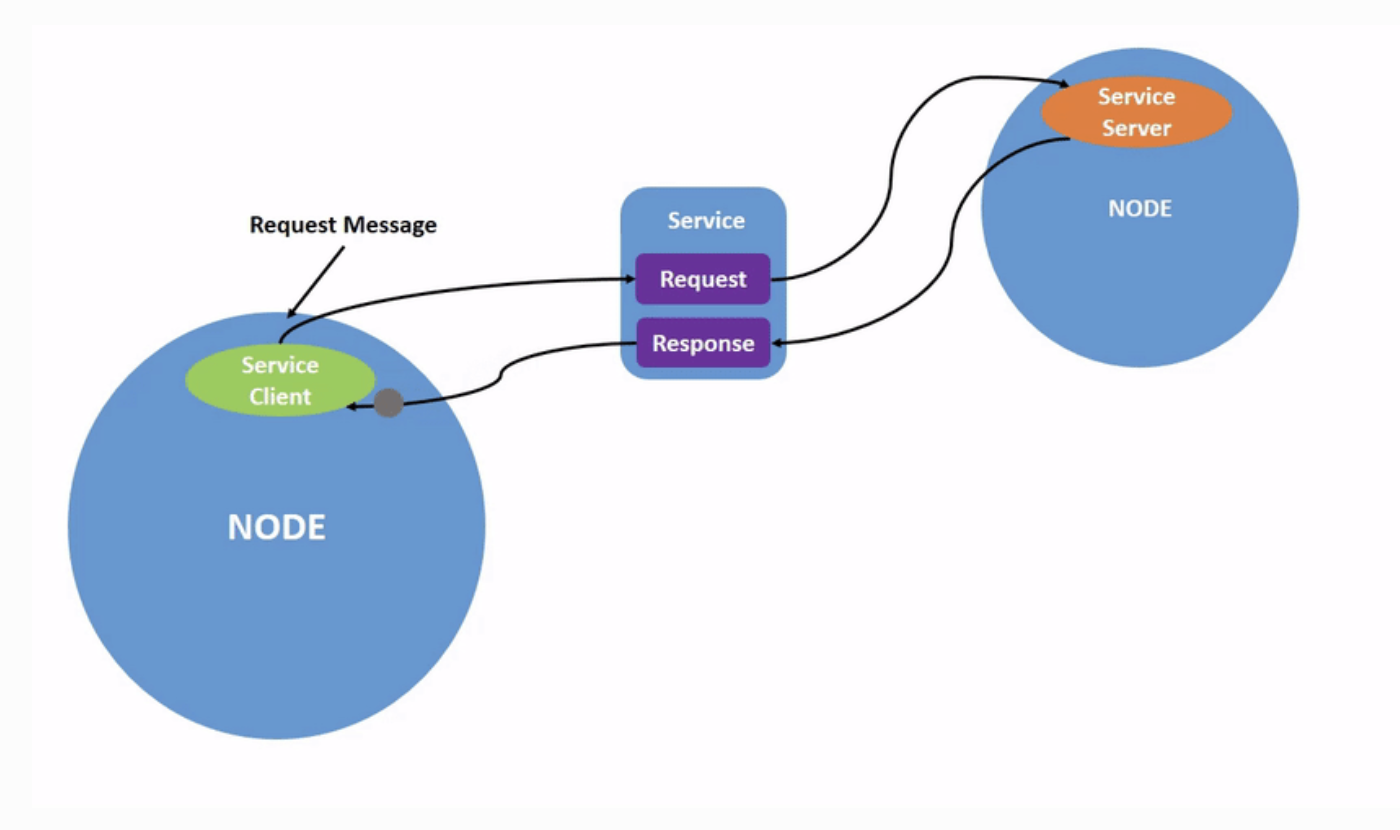
\includegraphics[width=\textwidth]{img/Services/Service_Wiki.png}
    \caption{Service Flowchart \textsuperscript{\ref{Services}}}
    \label{fig:sample}
\end{figure}

\paragraph{ros2 service list}~\\
We will now utilize the turtlesim simulator to gain a deeper understanding of how services function and how they can be used to our advantage. Open two separate terminals and run turtlesim\_node as well as turtle\_teleop\_key from the turtlesim package. A convenient method to list all currently available services is by using the command \texttt{ros2 service list}.

{\lstconsolestyle
\begin{lstlisting}
$ ros2 service list
/clear
/kill
/reset
/spawn
/teleop_turtle/describe_parameters
/teleop_turtle/get_parameter_types
/teleop_turtle/get_parameters
/teleop_turtle/list_parameters
/teleop_turtle/set_parameters
/teleop_turtle/set_parameters_atomically
/turtle1/set_pen
/turtle1/teleport_absolute
/turtle1/teleport_relative
/turtlesim/describe_parameters
/turtlesim/get_parameter_types
/turtlesim/get_parameters
/turtlesim/list_parameters
/turtlesim/set_parameters
/turtlesim/set_parameters_atomically
\end{lstlisting}}

\paragraph{ros2 service type}~\\
Just like topics have different message types, services have a corresponding interface known as the service type. For instance, the /clear service is used to erase all the previous traces left behind by the turtle. To determine the service type of a specific service, you can use the command \texttt{ros2 service type <service\_name>}.

{\lstconsolestyle
\begin{lstlisting}
$ ros2 service type /clear
std_srvs/srv/Empty
\end{lstlisting}}

\paragraph{ros2 service list}~\\
However, there's another convenient method to display all service types of available services using the \texttt{ros2 service list} command along with a specific flag. If you require additional information about a particular ros2 command, you can always utilize the \texttt{-h} or \texttt{--help} flag to access further details.
{\lstconsolestyle
\begin{lstlisting}
$ ros2 service list --help
usage: ros2 service list [-h] [--spin-time SPIN_TIME] [-s] [--no-daemon] [-t] [-c]
                         [--include-hidden-services]

Output a list of available services

options:
  -h, --help            show this help message and exit
  --spin-time SPIN_TIME
                        Spin time in seconds to wait for discovery (only applies when not using an
                        already running daemon)
  -s, --use-sim-time    Enable ROS simulation time
  --no-daemon           Do not spawn nor use an already running daemon
  -t, --show-types      Additionally show the service type
  -c, --count-services  Only display the number of services discovered
  --include-hidden-services
                        Consider hidden services as well
\end{lstlisting}}

\noindent
As you can see, this command provides the option to display the service types as well, using the \texttt{-t} or \texttt{--show-types} flag.
{\lstconsolestyle
\begin{lstlisting}
$ ros2 service list -t
/clear [std_srvs/srv/Empty]
/kill [turtlesim/srv/Kill]
/reset [std_srvs/srv/Empty]
/spawn [turtlesim/srv/Spawn]
/teleop_turtle/describe_parameters [rcl_interfaces/srv/DescribeParameters]
/teleop_turtle/get_parameter_types [rcl_interfaces/srv/GetParameterTypes]
/teleop_turtle/get_parameters [rcl_interfaces/srv/GetParameters]
/teleop_turtle/list_parameters [rcl_interfaces/srv/ListParameters]
/teleop_turtle/set_parameters [rcl_interfaces/srv/SetParameters]
/teleop_turtle/set_parameters_atomically [rcl_interfaces/srv/SetParametersAtomically]
/turtle1/set_pen [turtlesim/srv/SetPen]
/turtle1/teleport_absolute [turtlesim/srv/TeleportAbsolute]
/turtle1/teleport_relative [turtlesim/srv/TeleportRelative]
/turtlesim/describe_parameters [rcl_interfaces/srv/DescribeParameters]
/turtlesim/get_parameter_types [rcl_interfaces/srv/GetParameterTypes]
/turtlesim/get_parameters [rcl_interfaces/srv/GetParameters]
/turtlesim/list_parameters [rcl_interfaces/srv/ListParameters]
/turtlesim/set_parameters [rcl_interfaces/srv/SetParameters]
/turtlesim/set_parameters_atomically [rcl_interfaces/srv/SetParametersAtomically]
\end{lstlisting}}

\paragraph{ros2 interface show}~\\
The /clear command is shown to use the std\_srvs/srv/Empty service type. To visualize the structure of a service type, you can use the same command as you do for message types: \texttt{ros2 interface show <interface type>}. The typical structure of a service is as follows:
\begin{lstlisting}
data_type request_a
data_type request_b
---
data_type response
\end{lstlisting}

\noindent
Typically, the service type structure is divided into an upper and a lower half, separated by these three lines. The upper half signifies the inputs, while the lower half represents the outputs. Each input or output is associated with a specific data type. So let us have a further look at the service /clear.

{\lstconsolestyle
\begin{lstlisting}
$ros2 interface show std_srvs/srv/Empty 
---
\end{lstlisting}}

\noindent
The response of our command only returns three lines. This is due to the fact that this service doesn't require any input or output to clear the trails of the turtle. Such services are commonly utilized for settings such as turning on or shutting down an electric motor. In contrast, let's examine the /spawn service.


{\lstconsolestyle
\begin{lstlisting}
$ ros2 service type /spawn 
turtlesim/srv/Spawn
$ ros2 interface show turtlesim/srv/Spawn 
float32 x
float32 y
float32 theta
string name # Optional.  A unique name will be created and returned if this is empty
---
string name
\end{lstlisting}}

\noindent
As you can see, the service contains the four requests, x, y, theta and name and returns the name as a response.

\paragraph{ros2 service call}~\\
Now, we will proceed to call both services through our console. The command to call a service is \texttt{ros2 service call $<$service\_type$>$ $<$service\_type$>$ $<$request\_data$>$}. The request\_data follows the same YAML syntax as publishing a message. In your teleop\_turtle terminal, use your keyboard to navigate the turtle (trails need to be present to remove them). Next, we will call the /clear service to erase these trails.

{\lstconsolestyle
\begin{lstlisting}
$ ros2 service call /clear std_srvs/srv/Empty 
requester: making request: std_srvs.srv.Empty_Request()

response:
std_srvs.srv.Empty_Response()
\end{lstlisting}}

\noindent
After calling the service, all lines should have been removed. We will now call the /spawn command to get a second turtle. 

{\lstconsolestyle
\begin{lstlisting}
$ ros2 service call /spawn turtlesim/srv/Spawn "{x: 1.0, y: 1.0, name: 'olive_turtle'}"
requester: making request: turtlesim.srv.Spawn_Request(x=1.0, y=1.0, theta=0.0, name='olive_turtle')

response:
turtlesim.srv.Spawn_Response(name='olive_turtle')
\end{lstlisting}}

\noindent
After calling the service, another turtle with the name \texttt{olive\_turtle} spawns at the coordinates \texttt{x = 1.0} and \texttt{y = 1.0}. The turtle's name has an impact on the naming of its associated topics.

\paragraph{exercise}
\begin{enumerate}
    \item[$\bullet$] Utilize the command \texttt{ros2 topic list} to observe how the name influences the naming of topics.
    
    \item[$\bullet$] Test what happens if you spawn a turtle without specifying a name, considering that this option is optional.

    \item[$\bullet$] What happens if you spawn several turtles with the same name?
\end{enumerate}

\paragraph{RQt Service Caller}~\\
In the next step, we will once again utilize RQt, but this time to call a service. Open RQt and navigate to \texttt{Plugins $>$ Services $>$ Service Caller} to access the Service Caller tool. Choose the /spawn service, input the desired x, y, and theta values in the expression column, and then click the \texttt{Call} button to call the service. Similar to calling the service from the console, this action will result in the appearance of another turtle within the simulation.

\begin{figure}[H]
            \centering
            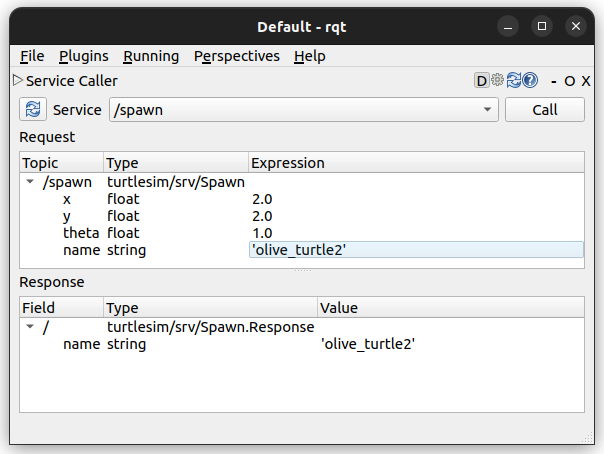
\includegraphics[width=  \textwidth]{img/Services/service_caller_spawn.png}
            \caption{RQt Service Caller}
\end{figure}

\paragraph{exercises}~\\
For the following tasks, attempt to call the services once from the terminal and then again using the Service Caller.

\begin{enumerate}
    \item[$\bullet$] Call \texttt{/kill} service to remove a turtle from the turtlesim screen. Spawn a turtle, and then use the kill service to make it disappear.

    \item[$\bullet$] Call the \texttt{/teleport\_absolute} service to teleport the turtle to another position on the screen.
\end{enumerate}


\subsubsection[Writing a Service Server and Client]{Writing a Service Server and Client\footnote{https://docs.ros.org/en/foxy/Tutorials/Beginner-Client-Libraries/Writing-A-Simple-Py-Publisher-And-Subscriber.html}}


After gaining an understanding of how services function, we will proceed with creating our own service client and server. Our objective is to develop a service that receives a temperature value in Celsius as a request and returns equivalent values in Kelvin and Fahrenheit. The following equations \footnote{\label{eq: temperature_equation}https://www.umrechnung.org/masseinheiten-temperatur-celsius-fahrenheit-kelvin/celsius-fahrenheit-umrechnung.htm} are used to calculate the Temperature from Celsius (\si{\degree}C) to Fahrenheit (\si{\degree}F) and Kelvin (K).

\begin{equation}
    \label{eq:Fahrenheit}
    \si{\degree}F = (\si{\degree}C \cdot \frac{9}{5}) + 32\si{\degree}
\end{equation}

\begin{equation}
    \label{eq:Kelvin}
    K = \si{\degree}C + 273.15
\end{equation}

\paragraph{Create an interface package} ~\\
Until now, we've been fortunate to work with msg and srv files that were already available. However, for our current task, it is required to use a custom-made srv file. Since the process for creating both msg and srv files is quite similar, we'll take this opportunity to create both. Up to this point, we only used \texttt{ament\_python} to build our packages. However, for creating packages involving interfaces, we need to use a CMake package. Before we proceed with creating the package, open a new terminal and navigate to the src folder as usual. To generate the \texttt{olive\_interfaces} package, we need to execute the \texttt{ros2 pkg create} command, specifying the build type as \texttt{ament\_cmake} to create a CMake package. Within this new package, create two directories: \texttt{msg} and \texttt{srv}. These directories will contain the message and service interfaces we'll be generating.

{\lstconsolestyle
\begin{lstlisting}
$ cd ~/Workspaces/ros2_olive_ws/src/
$ ros2 pkg create --build-type ament_cmake olive_interfaces
$ ls
$ cd olive_interfaces
CMakeLists.txt  include  package.xml  src
$ mkdir msg srv
$ ls
CMakeLists.txt  include  msg  package.xml  src  srv
\end{lstlisting}}

\paragraph[Custom msg interface]{Custom msg interface\footnote{https://docs.ros.org/en/foxy/Tutorials/Beginner-Client-Libraries/Custom-ROS2-Interfaces.html}}~\\
Let's begin by creating a message type designed to transmit RGB colour values using 8-bit unsigned integer values for each component. Please note that this message type is only created for demonstration purposes and won't be utilized in other projects. To proceed, navigate to your newly created msg folder using your terminal, then generate a file named \texttt{RGBColor.msg} and open it in a text editor.

{\lstconsolestyle
\begin{lstlisting}
$ cd msg
$ code RGBColor.msg
\end{lstlisting}}

\noindent
The typical structure of a message type involves listing the field type for each message value, followed by its name. It is important to note that the name has to start with a lowercase letter and must be composed of lowercase letters, digits, and underscores. You can find more comprehensive information about ROS2 interfaces at the provided link\footnote{https://docs.ros.org/en/humble/Concepts/Basic/About-Interfaces.html}. Now, let's revert to our RGB example. As we've chosen 8-bit unsigned integer field types for our red (r), green (g), and blue (b) values, our interface definition is as follows:

\begin{lstlisting}
uint8 r
uint8 g
uint8 b
\end{lstlisting}

\paragraph{CMakeLists.txt} ~\\
Before we proceed to build our package in order to make use of our newly created message interface, we need to make some preparations. This step involves editing the \texttt{CMakeLists.txt} and \texttt{package.xml} files. The \texttt{CMakeLists.txt} in a CMake package serves a similar purpose as the \texttt{setup.py} files do for Python packages. Let's start by including the following lines in our \texttt{CMakeLists.txt}
 file:

{\lstconsolestyle
\begin{lstlisting}
$ cd ..
$ code CMakeLists.txt
\end{lstlisting}}

\begin{lstlisting}
find_package(rosidl_default_generators REQUIRED)

rosidl_generate_interfaces(${PROJECT_NAME}
  "msg/RGBColor.msg"
  )
\end{lstlisting}

\noindent
The \texttt{find\_package} command within a CMake file is utilized to locate and configure external dependencies that our package depends on. Adding the \texttt{REQUIRED} keyword ensures that the specified package is available before attempting to build the package. The \texttt{rosidl} repository defines the message IDL (Interface Definition Language) syntax. We use one of its packages called \texttt{rosidl\_default\_generators} to generate our ROS2 interfaces. When generating interfaces, we need to append \texttt{$<$interface\_path$>$} after \texttt{\${PROJECT\_NAME}} for each new interface we wish to add to our package. In case you create an interface that depends on another interface, take a look at the ROS2 docs\footnote{https://docs.ros.org/en/humble/Tutorials/Beginner-Client-Libraries/Custom-ROS2-Interfaces.html}.

\paragraph{package.xml} ~\\
As the interfaces we aim to create depend on \texttt{rosidl\_default\_generators} for generating language-specific code, we need to specify a build tool dependency on it. \texttt{rosidl\_default\_runtime} serves as a runtime or execution-stage dependency required for utilizing these interfaces later on. Since we created this package just to declare new interfaces, we should also include it as a member of the \texttt{rosidl\_interface\_packages} group.

{\lstconsolestyle
\begin{lstlisting}
$ cd ~/Workspaces/ros2_olive_ws/src/olive_interfaces/
$ code package.xml
\end{lstlisting}}

\begin{lstlisting}
<buildtool_depend>rosidl_default_generators</buildtool_depend>
<exec_depend>rosidl_default_runtime</exec_depend>
<member_of_group>rosidl_interface_packages</member_of_group>
\end{lstlisting}

\paragraph{Test our new interface}~\\
Now, we are prepared to build our package. To achieve this, open a new terminal, navigate to the root of your workspace, and input the command \texttt{colcon build --packages-select olive\_interfaces}. Once you've sourced your terminal to the workspace, you can test if ROS 2 detects the new interface by running the \texttt{ros2 interface show} command.

{\lstconsolestyle
\begin{lstlisting}
    $ cd ~/Workspaces/ros2_olive_ws/
    $ source install/setup.bash
    $ ros2 interface show olive_interfaces/msg/RGBColor 
    
    uint8 r
    uint8 g
    uint8 b
\end{lstlisting}}

\paragraph{Custom srv interface} ~\\
Given that our primary objective at the moment is to develop the temperature service, we need to create the custom .srv file required for this task. This step closely resembles creating the msg interface. In your terminal, navigate to the \texttt{srv} folder of your \texttt{olive\_interfaces} package and create a new file with the name \texttt{TempConv.srv}. Since we want our input and output to be floating point values, we add the following lines to this file.

\begin{lstlisting}
# input: temperature in Celsius,   output: temperature in Kelvin
# and Fahrenheit
float64 temp_c
---
float64 temp_k
float64 temp_f
\end{lstlisting}

\paragraph{CMakeList.txt}~\\
It's important to recall that three lines separate the request and response of a service. For each new interface, there's no need to modify the package.xml file, but you do need to include the path to \texttt{rosidl\_generate\_interfaces} inside the \texttt{CMakeList.txt} file.

\begin{lstlisting}
rosidl_generate_interfaces(${PROJECT_NAME}
  "msg/RGBColor.msg"
  "srv/TempConv.srv"
  )
\end{lstlisting}

\paragraph{Testing the srv interface}~\\
Similar to the approach we used for messages, we can validate the new service interface by building the workspace, sourcing it, and then executing the command \texttt{ros2 interface show}.

{\lstconsolestyle
\begin{lstlisting}
    $ cd ~/Workspaces/ros2_olive_ws/
    $ colcon build --packages-select olive_interfaces
    $ source install/setup.bash
    $ ros2 interface show olive_interfaces/srv/TempConv 
    # input: temperature in Celsius,   output: temperature in Kelvin and Fahrenheit
    float64 temp_c
    ---
    float64 temp_k
    float64 temp_f
\end{lstlisting}
}

\subsubsection{Creating Service Server and Client}
\paragraph{Creating a Service Server}\footnote{https://docs.ros.org/en/humble/Tutorials/Beginner-Client-Libraries/Custom-ROS2-Interfaces.html}~\\
To construct our service client and service server, we will create a new package with the ament\_python build type. When generating new packages, it's often beneficial to add the \texttt{--dependencies} option to automatically include dependencies in your \texttt{package.xml} file. These dependencies will be listed as \texttt{$<$depend$>$dependency$<$/depend$>$}. It's important to note that using \texttt{$<$depend$>$} adds the dependency as both a build and execution dependency simultaneously. If, for instance, you want a just execution dependency, you have to change it manually this way. You can find further details about how \texttt{rosdep} manages dependencies at the provided link  \footnote{https://docs.ros.org/en/humble/Tutorials/Intermediate/Rosdep.html}. Given that we will require \texttt{rclpy} and \texttt{olive\_interfaces} for this project, we will integrate them while creating the new package using the following command:

{\lstconsolestyle
\begin{lstlisting}
$ cd ~/Workspaces/ros2_olive_ws/src/
$ ros2 pkg create olive_srvcli --build-type ament_python --dependencies rclpy olive_interfaces
\end{lstlisting}
}

\noindent
Similar to creating custom scripts for topics, we'll create scripts for our service client and server within the $<$package\_name$>$-folder (olive\_srvcli) of the new package. We'll begin by coding the server node in a new Python script named \texttt{service\_temperature.py}.

{\lstconsolestyle
\begin{lstlisting}
$ pwd
/home/fabian/Workspaces/ros2_olive_ws/src/olive_srvcli
$ cd olive_srvcli
$ code service_temperature.py
\end{lstlisting}
}

\begin{minted}{python}
import rclpy
from rclpy.node import Node
from olive_interfaces.srv import TempConv  
\end{minted}

\noindent
In our first block of code, we import all the necessary modules for our server node.

\begin{minted}{python}
class TempService(Node):

    def __init__(self):
        super().__init__('temp_service')
        self.srv = self.create_service(TempConv, 'temp_conversion', 
        self.temp_conversion_callback)

    def temp_conversion_callback(self, request, response):
        response.temp_k = request.temp_c + 273.15
        response.temp_f = (request.temp_c * 9 / 2) + 32
        self.get_logger().info(
                f'Incoming request \n Temperature in Celsius: {request.temp_c}'
                )
        return response
\end{minted}

\noindent
In this block, we initialize our server node and call the \texttt{create\_service(srv\_type, srv\_name, callback)} function to create a service. As \texttt{srv\_type}, we choose \texttt{TempConv} to call our service \texttt{temp\_conversion}. \texttt{temp\_conversion\_callback} is the callback function of the service. It will be executed whenever a service is called. The callback function is where the actual service logic is implemented, and it takes the two arguments, request and response. Remember that the service definition for \texttt{TempConv} had the request \texttt{temp\_c} and the responses \texttt{temp\_k} and \texttt{temp\_f}. We use the formulas (\ref{eq:Fahrenheit}) and (\ref{eq:Kelvin}) to compute our response values. In addition, printing them to the terminal is always a good way to ensure the system is working.

\begin{minted}{python}
def main():
    rclpy.init()
    temp_service = TempService()
    rclpy.spin(temp_service)
    rclpy.shutdown
    
if __name__ == '__main__':
    main()
\end{minted}

\noindent
The last block is similar to previous scripts. \\
Because we declared our dependency already while creating our package, we just have to add an entry point in the setup.py file. To do this, add the following lines between the \texttt{console\_scripts} brackets:

\begin{lstlisting}
    'temp_server = olive_srvcli.service_temperature:main',
\end{lstlisting}


\paragraph{Creating a Service Client}\footnote{https://docs.ros.org/en/humble/Tutorials/Beginner-Client-Libraries/Custom-ROS2-Interfaces.html}~\\

\noindent
Our next step is to create a client node that is able to call our server node. Since we need a request in Celsius for our client, we will implement an input using the python \texttt{sys} library. It enables us to get user input from the command line using argv, which is comparable to C. If you don't know how this works, it is recommended to take a look at the following source \footnote{https://www.knowledgehut.com/blog/programming/sys-argv-python-examples\#key-takeaways\%C2\%A0 }. For our client, create a new file called \texttt{client\_temperature.py} and open it in a code editor.

\begin{minted}{python}
import rclpy
from rclpy.node import Node
import sys
from olive_interfaces.srv import TempConv    
\end{minted}

\noindent
In addition to before, we have to import the sys library for the command line input.

\begin{minted}{python}
class TempClient(Node):

    def __init__(self):
        super().__init__('temp_client')
        self.cli = self.create_client(TempConv, 'temp_conversion')
        while not self.cli.wait_for_service(timeout_sec=1.0):
            self.get_logger().info('service not available, waiting again..')
        self.req = TempConv.Request()

    def send_request(self, temp_c):
        self.req.temp_c = temp_c
        self.future = self.cli.call_async(self.req)
        rclpy.spin_until_future_complete(self, self.future)
        return self.future.result()
\end{minted}
To create a client, we use the \texttt{create\_client} command, which takes the service type and the service name as input. The \texttt{wait\_for\_service} method is called on the service client to wait for the service to become available. It takes an optional argument\texttt{ timeout\_sec}, which specifies the maximum amount of time (in seconds) to wait for the service before giving up. In this case, \texttt{timeout\_sec=1.0} indicates that the client will wait for up to 1 second. The created while loop will run until the service is available and print feedback to the terminal. We must also initialize a request object of the \texttt{TempConv} Service type that will be used for our other function.\\

\noindent
In addition to our \texttt{\_\_init\_\_} function, we define a send\_request function in our class that will be used to send the request later, as the name suggests. We have our request (\texttt{temp\_c}) as input of the function. It is stored inside the request object we initialized before. The \texttt{rclpy} function \texttt{call\_async} takes a request as input and returns a future object that completes as soon as the request completes\footnote{https://docs.ros2.org/foxy/api/rclpy/api/services.html}.\\
\noindent
A future represents an eventual result of an asynchronous operation. Future objects are used to bridge low-level callback-based code with high-level async/await code\footnote{https://docs.python.org/3/library/asyncio-future.html}. This concept is important for the communication between both the client and the server node. We use the \texttt{spin\_until\_future\_complete} command to spin our node until the future is complete, or in other words, until the server sets both response values (\texttt{temp\_k}, \texttt{temp\_f}). In the end, we return the result of the future, the response.
\begin{minted}{python}
def main():
    rclpy.init()
    temp_client = TempClient()
    response = temp_client.send_request(float(sys.argv[1]))
    temp_client.get_logger().info(
    f'The Temperature of {float(sys.argv[1])} Celsius is equal to {response.temp_k} 
    Kelvin and {response.temp_f} Fahrenheit'
    )
    temp_client.destroy_node()
    rclpy.shutdown()

if __name__ == '__main__':
    main()
\end{minted}

\noindent
This is the moment we use the command line input(argv) to send the request to the server. The rest of the code is similar to previous scripts.\\
Just as before, we have to add the following lines to our \texttt{setup.py} file to set our entry point.
\begin{lstlisting}
    'temp_client = olive_srvcli.client_temperature:main',
\end{lstlisting}

\noindent
In the end, we want to verify everything is working as expected. In a console, navigate to the root of your workspace and build it. Run both scripts in two separate terminals after sourcing the workspace, and remember to add an input argument for the client command. 

{\lstconsolestyle
\begin{lstlisting}
$ cd ~/Workspaces/ros2_olive_ws/
$ colcon build --symlink-install --packages-select olive_srvcli
$ source install/setup.bash
$ ros2 run olive_srvcli temp_server 
[INFO] [1692882087.750895743] [minimal_service]: Incoming request 
 Temperature in Celsius: 0.0
 \end{lstlisting}

\begin{lstlisting}
$ source ~/Workspaces/ros2_olive_ws/install/setup.bash
$ ros2 run olive_srvcli temp_client 0.0
[INFO] [1692882034.999264266] [temp_client]: service not available, waiting again..
[INFO] [1692882036.001810124] [temp_client]: service not available, waiting again..
[INFO] [1692882087.751789540] [temp_client]: The Temperature of 0.0 Celsius is equal to 273.15 Kelvin and 32.0 Fahrenheit
 \end{lstlisting}
 }

\paragraph{exercise}~\\
Choose one of the following exercises.
\begin{enumerate}
    \item[$\bullet$] Create a client and server. The client has to send a request for money in euros to the service and should get the equivalent value in three different currencies in return. (e.g. dollar, pound, Swiss franc)
    \item[$\bullet$] Create a client and server. The client has to send a request for an integer to the service and should get the factorial of this value in return.
\end{enumerate}


\subsection{Working with Parameters}
A parameter is a configuration value of a node. Parameters affect the node's behaviour at startup and runtime. Think of them like the settings of a node. Parameters in ROS 2 can have different data types, including integers, floats, booleans, strings and lists.\\

\subsubsection[Params in Turtlesim]{Params in Turtlesim\footnote{https://docs.ros.org/en/foxy/Tutorials/Beginner-CLI-Tools/Understanding-ROS2-Parameters/Understanding-ROS2-Parameters.html}}
\noindent
We will now use the turtlesim simulator again to get a further understanding of how parameters work and how we can use them to our advantage in robotic systems.\\

\noindent
From the turtlesim package, run \texttt{turtlesim\_node} and \texttt{turtle\_teleop\_key} in two separate terminals. To see which parameters are currently available, we use the command \texttt{ros2 param list} in another terminal. This command can be used to list all nodes and the parameters that are part of that node.

{\lstconsolestyle
\begin{lstlisting}
$ ros2 param list
/teleop_turtle:
  qos_overrides./parameter_events.publisher.depth
  qos_overrides./parameter_events.publisher.durability
  qos_overrides./parameter_events.publisher.history
  qos_overrides./parameter_events.publisher.reliability
  scale_angular
  scale_linear
  use_sim_time
/turtlesim:
  background_b
  background_g
  background_r
  qos_overrides./parameter_events.publisher.depth
  qos_overrides./parameter_events.publisher.durability
  qos_overrides./parameter_events.publisher.history
  qos_overrides./parameter_events.publisher.reliability
  use_sim_time
\end{lstlisting}
}

\noindent
The turtlesim parameters background\_b, background\_g and background\_c contain the RGB values of the simulation background color. It is possible to get each of those values with the \texttt{ros2 param get $<$node$>$ $<$node\_parameter$>$} command.

{\lstconsolestyle
\begin{lstlisting}
$ ros2 param get /turtlesim background_r
Integer value is: 69
$ ros2 param get /turtlesim background_g
Integer value is: 86
$ ros2 param get /turtlesim background_b
Integer value is: 255
\end{lstlisting}
}

\noindent
The standard parameter values for the simulation are red: 69, green: 89 and blue: 255. For the task of changing parameters, use the commmand \texttt{ros2 param set $<$node$>$ $<$node\_parameter$>$ $<$parameter\_value$>$}. For now, we want to change the red value of the background colour to 255 (the highest value).

{\lstconsolestyle
\begin{lstlisting}
$ ros2 param set /turtlesim background_r 255
Set parameter successful
\end{lstlisting}
}

\noindent
The background colour changes instantly to purple since parameters change nodes' behaviour during runtime, as already said.\\

\newpage
\paragraph{exercise}~\\
\begin{enumerate}
    \item[$\bullet$] Change the background colour to yellow.
    \item[$\bullet$] Change the background colour to black.
\end{enumerate}

\paragraph{Use files to save parameters}~\\
In ROS2, it is possible to use YAML files to save parameter settings. The content that will be inside that file can be displayed by using the \texttt{ros2 param dump $<$node\_name$>$} command. We will now use this command for the \texttt{/turtlesim} node.

{\lstconsolestyle
\begin{lstlisting}
$ ros2 param dump /turtlesim 
/turtlesim:
  ros__parameters:
    background_b: 255
    background_g: 86
    background_r: 255
    qos_overrides:
      /parameter_events:
        publisher:
          depth: 1000
          durability: volatile
          history: keep_last
          reliability: reliable
    use_sim_time: false
\end{lstlisting}
}

\noindent
To dump the parameters to a YAML file, we have to append \texttt{ $>$ file\_name} to the end of the command. It is important to note that this file will be placed inside your current directory. So, before using the command, make sure to navigate to the folder you want to place your file. For demonstration purposes, we are going to use the \texttt{Documents} folder for this task.

{\lstconsolestyle
\begin{lstlisting}
$ cd ~/Documents/
$ ros2 param dump /turtlesim > turtlesim.yaml
$ code turtlesim.yaml
\end{lstlisting}
}

\noindent
After opening the file, you will see that the same content as before has been placed inside the new file. You can change the content of this file however you want to set the parameters and load it to apply the changes to your node. Before we load the file again, we must change the values inside it to be able to spot the difference (e.g. 0/0/0). The command to load the parameters from a file is \texttt{ros2 param load $<$node\_name$>$ $<$document\_name$>$}.

{\lstconsolestyle
\begin{lstlisting}
$ ros2 param load /turtlesim turtlesim.yaml
\end{lstlisting}
}

\noindent
The changes will be applied directly after loading our parameter file. \\

\noindent
It is also possible to start a node with the parameters of a file by adding \texttt{--ros-args --params-file $<$file\_name$>$} at the end of your ros2 run command. If you use \texttt{ros2 run turtlesim turtlesim\_node --ros-args --params-file turtlesim.yaml}, a new instance of turtlesim opens with the custom parameters of the YAML file.


\subsubsection[Using Parameters in a Class]{Using Parameters in a Class\footnote{https://docs.ros.org/en/foxy/Tutorials/Beginner-Client-Libraries/Using-Parameters-In-A-Class-Python.html}}
So far, we only used parameters that were already available to use. But if we want to create our own robotic projects, we have to learn how we can create parameters inside a class. For this topic, we will create a parameter for our random number generator that allows us to adjust the upper limit of the generated numbers. Open your \texttt{random\_number\_publisher.py} file in a text editor.\\

\noindent
Inside the \texttt{\_\_intit\_\_} function of our class, we declare our parameter with the \texttt{declare\_parameter(name, value)} function. We call our parameter \texttt{upper\_limit} and set its standard value to 100.

\begin{minted}{python}
self.declare_parameter('upper_limit', 100)
\end{minted}

\noindent
Inside the \texttt{publish\_random\_number} function, we declare a variable \texttt{upper\_limit} that gets the current parameter value from the \texttt{get\_parameter} function. The last change is to replace the old upper limit (100) with the new variable for the upper limit inside the \texttt{randint} function.

\begin{minted}{python}
upper_limit = self.get_parameter('upper_limit').get_parameter_value().integer_value
random_number = random.randint(1, upper_limit)
\end{minted}

\noindent
Since we used \texttt{--symlink-install} to build the workspace previously, we can test our changes directly by running the node and changing the parameter from another terminal with the \texttt{ros2 param set} function.

{\lstconsolestyle
\begin{lstlisting}
$ ros2 run random_number_ps random_number_publisher 
[INFO] [1692974302.646532808] [random_number_publisher]: Publishing: 74
[INFO] [1692974303.636122165] [random_number_publisher]: Publishing: 35
[INFO] [1692974304.635955454] [random_number_publisher]: Publishing: 65
[INFO] [1692974406.809493888] [random_number_publisher]: Publishing: 614
[INFO] [1692974407.809362516] [random_number_publisher]: Publishing: 358
[INFO] [1692974408.809298156] [random_number_publisher]: Publishing: 319

\end{lstlisting}
}

{\lstconsolestyle
\begin{lstlisting}
$ ros2 param set /random_number_publisher upper_limit 1000
Set parameter successful
\end{lstlisting}
}

\paragraph{exercise}~\\
\begin{enumerate}
    \item[$\bullet$] Create a parameter to set the lower bound for the random number publisher.
\end{enumerate}

\subsection[Working with Actions]{Working with Actions\footnote{https://docs.ros.org/en/foxy/Tutorials/Beginner-CLI-Tools/Understanding-ROS2-Actions/Understanding-ROS2-Actions.html}}
The last important ROS2 interface is called actions. They consist of three separate parts and are used for long-running tasks. The goal message specifies what needs to be achieved, the feedback message is used to provide progress updates during runtime, and the result message holds the outcome of the action. If you have a client node that wants to achieve a specific goal, it sends a goal request to an action server. This server provides the client with constant feedback and returns the result as soon as the goal is completed.\\

\noindent
In two separate terminals, start the two nodes \texttt{/turtlesim} and \texttt{/teleop\_turtle}.
{\lstconsolestyle
\begin{lstlisting}
$ ros2 run turtlesim turtlesim_node
\end{lstlisting}
}
{\lstconsolestyle
\begin{lstlisting}
$ ros2 run turtlesim turtle_teleop_key
Reading from keyboard
---------------------------
Use arrow keys to move the turtle.
Use G|B|V|C|D|E|R|T keys to rotate to absolute orientations. 'F' to cancel a rotation.
'Q' to quit.

\end{lstlisting}
}

\noindent
We were already using the arrow keys to send messages, but the \texttt{teleop\_turtle} node is also able to send orientation goals with the keys surrounding the F key (E, R, T, D, G, C, V, B). The theta angle that is requested corresponds to the orientation of the key relative to F. For example, if we use the R key, which is right above F, we send the goal to change the orientation of the turtle to 90\si{\degree} or 1.57rad ($\pi / 2$). Use a key of your choice and pay attention to the \texttt{/turtlesim} monitor.

{\lstconsolestyle
\begin{lstlisting}
[INFO] [1693213924.173110078] [turtlesim]: Rotation goal completed successfully
\end{lstlisting}
}

\noindent
As soon as the goal is completed, the terminal tells us that the goal is completed. A critical property of actions is that a goal can be cancelled before a goal is finished. In comparison, services will finish their task and only accept new requests as soon as they have completed their tasks. To test this, press D, followed by G, before the goal is finished. You will see that the turtle is turning abruptly in the other direction. The \texttt{turtlesim} monitor will warn you in case a goal is aborted.

{\lstconsolestyle
\begin{lstlisting}
[WARN] [1693215047.805568573] [turtlesim]: Rotation goal received before a previous goal finished. Aborting previous goal
[INFO] [1693215050.653160327] [turtlesim]: Rotation goal completed successfully
\end{lstlisting}
}

\noindent
In this case, the server receives a new goal and decides to abort the current goal for this new goal. It is also possible to use the client to cancel a goal by pressing the F key. It is important to note that it depends on the action server if it aborts a goal or not when it gets a new one. \\

\noindent
We previously used \texttt{ros2 node info} to get a list of the different publishers and subscribers of a node. It is also helpful to get information about services and actions.

{\lstconsolestyle
{\begin{lstlisting}
$ ros2 node info /turtlesim 
/turtlesim
  (...)
  Action Servers:
    /turtle1/rotate_absolute: turtlesim/action/RotateAbsolute
  Action Clients:
\end{lstlisting}}

{\begin{lstlisting}
$ ros2 node info /teleop_turtle 
(...)
  Action Servers:
  Action Clients:
    /turtle1/rotate_absolute: turtlesim/action/RotateAbsolute
\end{lstlisting}}
}

\noindent
Notice that the \texttt{/teleop\_turtle} node is the client and \texttt{/turtlesim} the server of the \texttt{/turtle1/rotate\_absolute} action. In case you press a key in the \texttt{/teleop\_turtle monitor}, a goal request is sent to the \texttt{/turtle1/rotate\_absolute} action. The \texttt{/turtlesim} node will be responsible for responding to this request, providing feedback and returning the result after completion.\\
Just as with topics and services, you have to specify an interface type for actions. \\ \texttt{turtlesim/action/RotateAbsolute}, is the action type that is used for this action.\\
You can use the \texttt{ros2 action list} command to list all actions that are currently available. Similar to topics, you can use the -t flag to print the corresponding action types to the terminal.\\

{\lstconsolestyle
\begin{lstlisting}
$ ros2 action list -t
/turtle1/rotate_absolute [turtlesim/action/RotateAbsolute]
\end{lstlisting}
}

\noindent
Use \texttt{ros2 action info $<$action\_name$>$} to get specific information about the clients and the servers of an action.

{\lstconsolestyle
\begin{lstlisting}
$ ros2 action info /turtle1/rotate_absolute 
Action: /turtle1/rotate_absolute
Action clients: 1
    /teleop_turtle
Action servers: 1
    /turtlesim
\end{lstlisting}
}

\noindent
Before being able to send a custom goal, you have to be able to know how an action is structured. This task is just as easy as for the other interface types. Use \texttt{ros2 interface show $<$interface\_type$>$} to print the structure of a specific action to your terminal.

{\lstconsolestyle
\begin{lstlisting}
$ ros2 interface show turtlesim/action/RotateAbsolute 
# The desired heading in radians
float32 theta
---
# The angular displacement in radians to the starting position
float32 delta
---
# The remaining rotation in radians
float32 remaining
\end{lstlisting}
}

\noindent
Three lines separate the different sections. The first part represents the goal request. In this case, the theta angle for the orientation in radians. The second section is the result. It will be sent as soon as the task is completed, and for our example, it represents the angular displacement in radians to the starting position. The last part is for feedback that will be sent during the process. In our case, we can get the remaining rotation as feedback.\\

\noindent
Since we are now aware of action structures, we can use this to our advantage to send our own goals to an action server. We use the \texttt{ros2 action send\_goal $<$action\_name$>$ $<$action\_type$>$ $<$values$>$} command for this task. The $<$values$>$ part uses the YAML format, just like sending a message or calling an interface. We will now try to emulate pressing the D and G keys in the \texttt{/teleop\_turtle terminal}. D corresponds to an orientation of $theta =\pi \approx 3.141 rad$ and G to an orientation of $theta = 0 rad$. 

{\lstconsolestyle
\begin{lstlisting}
$ ros2 action send_goal /turtle1/rotate_absolute turtlesim/action/RotateAbsolute '{theta: 3.141}'
Waiting for an action server to become available...
Sending goal:
     theta: 3.141

Goal accepted with ID: 1cfd86b5fb284d1bbb0a5314313314bc

Result:
    delta: 3.119999885559082

Goal finished with status: SUCCEEDED
\end{lstlisting}
}

\noindent
In case we want to print the feedback for our request, we can use the \texttt{--feedback} flag for our command. We will continue to get feedback until the goal is completed.

{\lstconsolestyle
\begin{lstlisting}
$ ros2 action send_goal /turtle1/rotate_absolute turtlesim/action/RotateAbsolute '{theta: 0}' --feedback
(...)
Feedback:
    remaining: 0.02718530036509037

Feedback:
    remaining: 0.01118529960513115

Result:
    delta: -3.119999885559082

Goal finished with status: SUCCEEDED

\end{lstlisting}
}

\noindent
In this course, we will not discuss how we can create our own action node since this task is beyond the beginner level and not needed for this course. If you are still interested in how you can do it, take a look at the following link for more information\footnote{https://docs.ros.org/en/iron/Tutorials/Intermediate/Writing-an-Action-Server-Client/Py.html}.

\subsection[Using Launch Files]{Using Launch Files\footnote{https://docs.ros.org/en/humble/Tutorials/Intermediate/Launch/Creating-Launch-Files.html}}
In case you have a big project and a handful of executables, it is often annoying running them one by one in separate terminals. ROS2 provides a solution for this problem in the form of launch files that allow us to run different executables by just running one command. Launch files can additionally be used for other things like setting the starting parameters, but for now, this is not our primary objective. To keep things in order, it is convenient to store all launch files in a single directory. This folder is going to be part of a new package whose purpose is dedicated to launching. For now, this part is optional, as we start by running our launch files from the current directory. Later on, this package will be used to run our launch files directly from the package itself. Like always, navigate to the \texttt{src} folder before creating a new package. We already added \texttt{turtlesim} as a dependency since we are going to run two instances of \texttt{turtlesim\_node} for demonstration purposes. Within our new package, we first create our \texttt{launch} folder to store all of our launch files. We continue with creating our first launch file named \texttt{turtle\_launch.py}. In alternative to using Python for creating launch files, there is the option of using XML or YAML for this task.

{\lstconsolestyle
\begin{lstlisting}
$ cd ~/Workspaces/ros2_olive_ws/src
$ ros2 pkg create olive\_launch --dependencies turtlesim --build-type ament\_python
$ cd olive_launch
$ mkdir launch
$ cd launch
$ code turtle_launch.py
\end{lstlisting}
}

\begin{minted}{python}
from launch import LaunchDescription
 
def generate_launch_description():
    return LaunchDescription([
    ])
\end{minted}
\noindent
To initialize the launch description, we have to input a launch description entity, which is a list of several actions. Each action represents a specific behaviour or configuration that you want to apply during the launch process. To add an action that enables the launch file to start a node, we have to import the node action from the \texttt{launch\_ros.actions package}. For every node action, you are able to define things like names, namespaces, executables, parameters, packages, etc. For the first test, we initialize a node action to run the \texttt{turtlesim\_node} executable by adding the following lines to the launch description.

\begin{minted}{python}
Node(
    package='turtlesim',
    executable='turtlesim_node',
    name='turtle1',
),
\end{minted}

\noindent
We can test our launch file by running the \texttt{ros2 launch $<$launch\_file$>$} command inside our launch directory. 

{\lstconsolestyle
\begin{lstlisting}
$ cd ~/Workspaces/ros2_olive_ws/src/olive_launch/launch
$ ros2 launch turtle_launch.py
\end{lstlisting}
}

\noindent
After running the command, the turtlesim simulation starts as usual. Since this is the same as when using the \texttt{ros2 run} command, we are going to add a second \texttt{turtlesim\_node} to our launch file to prove the advantage of launch files for larger projects.

\begin{minted}{python}
Node(
    package='turtlesim',
    executable='turtlesim_node',
    name='turtle2',
),
\end{minted}

\noindent
Running the launch file a second time, launches two \texttt{turtlesim} windows at once.\\

\noindent
Since having to navigate to a specific folder to launch a file isn't really optimal, it is more common to use the \texttt{ros2 launch $<$package$>$ $<$launch\_file$>$} command. To be able to use this command, we have to make some changes inside our packages \texttt{setup.py file}.

\begin{minted}{python}
data_files=[
    (...),
    (os.path.join('share', package_name, 'launch'),
    glob(os.path.join('launch', '*launch.[pxy][yma]*')))
],
\end{minted}

\noindent
The data files argument in a setup.py file is used to specify additional files that should be included when the package is installed. Every element in \texttt{data\_files} is a tuple that consists of the installation path and source files. By adding the command, we make sure that all files inside our launch folder with a \texttt{py}, \texttt{yaml} or \texttt{xml} ending will be installed to share/package\_name/olive\_launch. Since we already added the dependency \texttt{turtlesim} while building the package, it is not essential to change the \texttt{package.xml} file, but in case you create a launch file that depends on another package, you should not forget to add the dependencies. After building the package again and sourcing our workspace, we are now able to launch our file from the \texttt{olive\_launch} package.

{\lstconsolestyle
\begin{lstlisting}
$ cd ~/Workspaces/ros2_olive_ws/
$ colcon build --symlink-install --packages-select olive_launch
$ source install/setup.bash
$ ros2 launch olive_launch turtle_launch.py
\end{lstlisting}
}


\paragraph{End of chapter}~\\
Using the information you've learned in this chapter, you are now capable of creating your own robotic projects. Since there are still a few topics that won't be covered in this course, if you're interested in further expanding your knowledge of ROS2, feel free to explore the official ROS2 docs\footnote{https://docs.ros.org/en/humble/}. In the next section, you will apply what you've learned using real robotic components from the Olive-Robotics OWL Kit. You can refer back to the previous chapters as reference material for the upcoming challenges in the course. You'll begin by working with individual components like the IMU and gradually progress to combining them into complex systems.
\newpage




\section{Owl Kit Projects}

Now that we have gotten a solid understanding of the fundamental concepts of ROS2, we have a strong foundation for building our first robotic system. We will begin by exploring the various components that the Olive Owl Kit provides, learning how to use each part individually. With the knowledge gained, we will then move on to the exciting task of integrating the modules into a complex robotic system.

\subsection{About the Owl Kit}
The OWL KIT\footnote{\label{docs:owl_kit}https://docs.olive-robotics.com/kits/owl/owl.html} (figure: \ref{fig:owl_kit}) is a kit containing different modular robotic components which we are going to utilize for building our own robot.
\begin{enumerate}
    \item[$\bullet$]2x olive® Servo OLV-SRV01-B32
    \item[$\bullet$]1x olive® IMU OLV-IMU01-9DB
    \item[$\bullet$]1x olive® Camera OLV-CAM01-TP
\end{enumerate}
Utilizing Olive Robotics hardware offers the advantage of simplicity. These components come pre-installed with ROS and ROS2, allowing us to integrate them by simply connecting cables seamlessly. This solution eliminates the need to spend time configuring communication between individual parts, making it ideal for applying the ROS2 fundamentals we've learned in the previous chapter.


\begin{figure}[H]
    \centering
    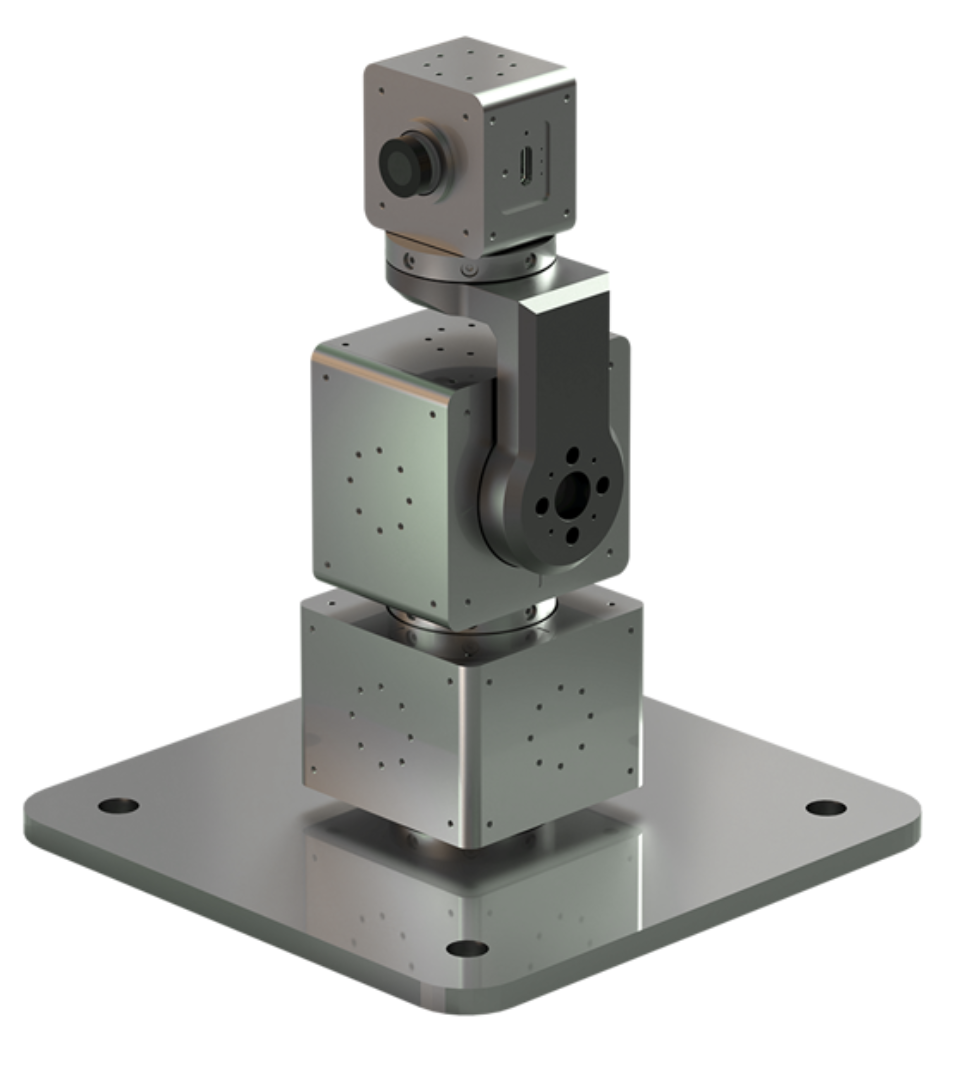
\includegraphics[width=0.5\textwidth]{img/owl_kit.png}
    \caption[Olive Robotics OWL KIT]{Olive Robotics OWL KIT\textsuperscript{\ref{docs:owl_kit}}}
    \label{fig:owl_kit}
\end{figure}


\subsection{Olive Docs}
Olive Robotics provides documentation\footnote{https://docs.olive-robotics.com/} for all of their components and software, which can be found in the link. This documentation contains all the necessary information to help us effectively use their products. To establish a connection between the Olive devices and your computer, you can refer to the quick-start guide provided in the documentation.\footnote{https://docs.olive-robotics.com/quick\_start.html}.\\
For now, we will follow this guide to establish the initial connection of our first module to our PC. To begin, take an IMU module and use a cable to connect it to your computer. Follow the instructions provided in the documentation and ensure that everything is functioning correctly by listing all the available topics.\\

\noindent
For instance, if you connect the Olive IMU module, the terminal will display the following output.
{\lstconsolestyle
\begin{lstlisting}
$ ros2 topic list
    /olive/imu/x1684267976913/imu
    /olive/imu/x1684267976913/led
    /olive/imu/x1684267976913/magnetometer
    /olive/imu/x1684267976913/status
    /olive/imu/x1684267976913/switch
    /olive/imu/x1684267976913/temperature
    /parameter_events
    /rosout

\end{lstlisting}
}  
\subsection{IMU}
The IMU module will be the first component we explore in greater detail. We will utilize it in our initial project to control the turtlesim turtle using its sensor data.

\subsubsection{What is an IMU}
The IMU\footnote{https://docs.olive-robotics.com/hardware/imu/imu.html} (Inertial Measurement Unit) is a versatile and compact sensor that provides precise orientation, acceleration, and angular rate measurements for robotic applications. In this course, we utilize Olives OLV-IMU01-13D\footnote{https://docs.olive-robotics.com/hardware/imu/imu\_01\_13d.html} (figure \ref{fig:olive_imu}) IMU, that consists of the following components.
\begin{enumerate}
    \item[$\bullet$]\texttt{3-axis gyroscope:} The IMU module features a 3-axis gyroscope that provides accurate and reliable angular rate data in all three dimensions (x, y, z). This allows you to measure the orientation of the IMU module with respect to a fixed reference frame and to track the changes in orientation over time.
    \item[$\bullet$]\texttt{3-axis accelerometer:} The IMU module also features a 3-axis accelerometer that provides accurate and reliable acceleration data in all three dimensions (x, y, z). This allows you to measure the linear acceleration of the IMU module with respect to a fixed reference frame and to track the changes in linear acceleration over time.
    \item[$\bullet$]\texttt{3-axis magnetometer:} The IMU module also features a 3-axis magnetometer that provides accurate and reliable magnetic field data in all three dimensions (x, y, z). This allows you to measure the magnetic field of the IMU module with respect to a fixed reference frame and to track the changes in the magnetic field over time.
    \item[$\bullet$]\texttt{4-measurements environmental sensor:} The barometer is an instrument used to measure atmospheric pressure, the presence which is the force exerted by the weight of the atmosphere on a given surface.
\end{enumerate}

\begin{figure}[H]
    \centering
    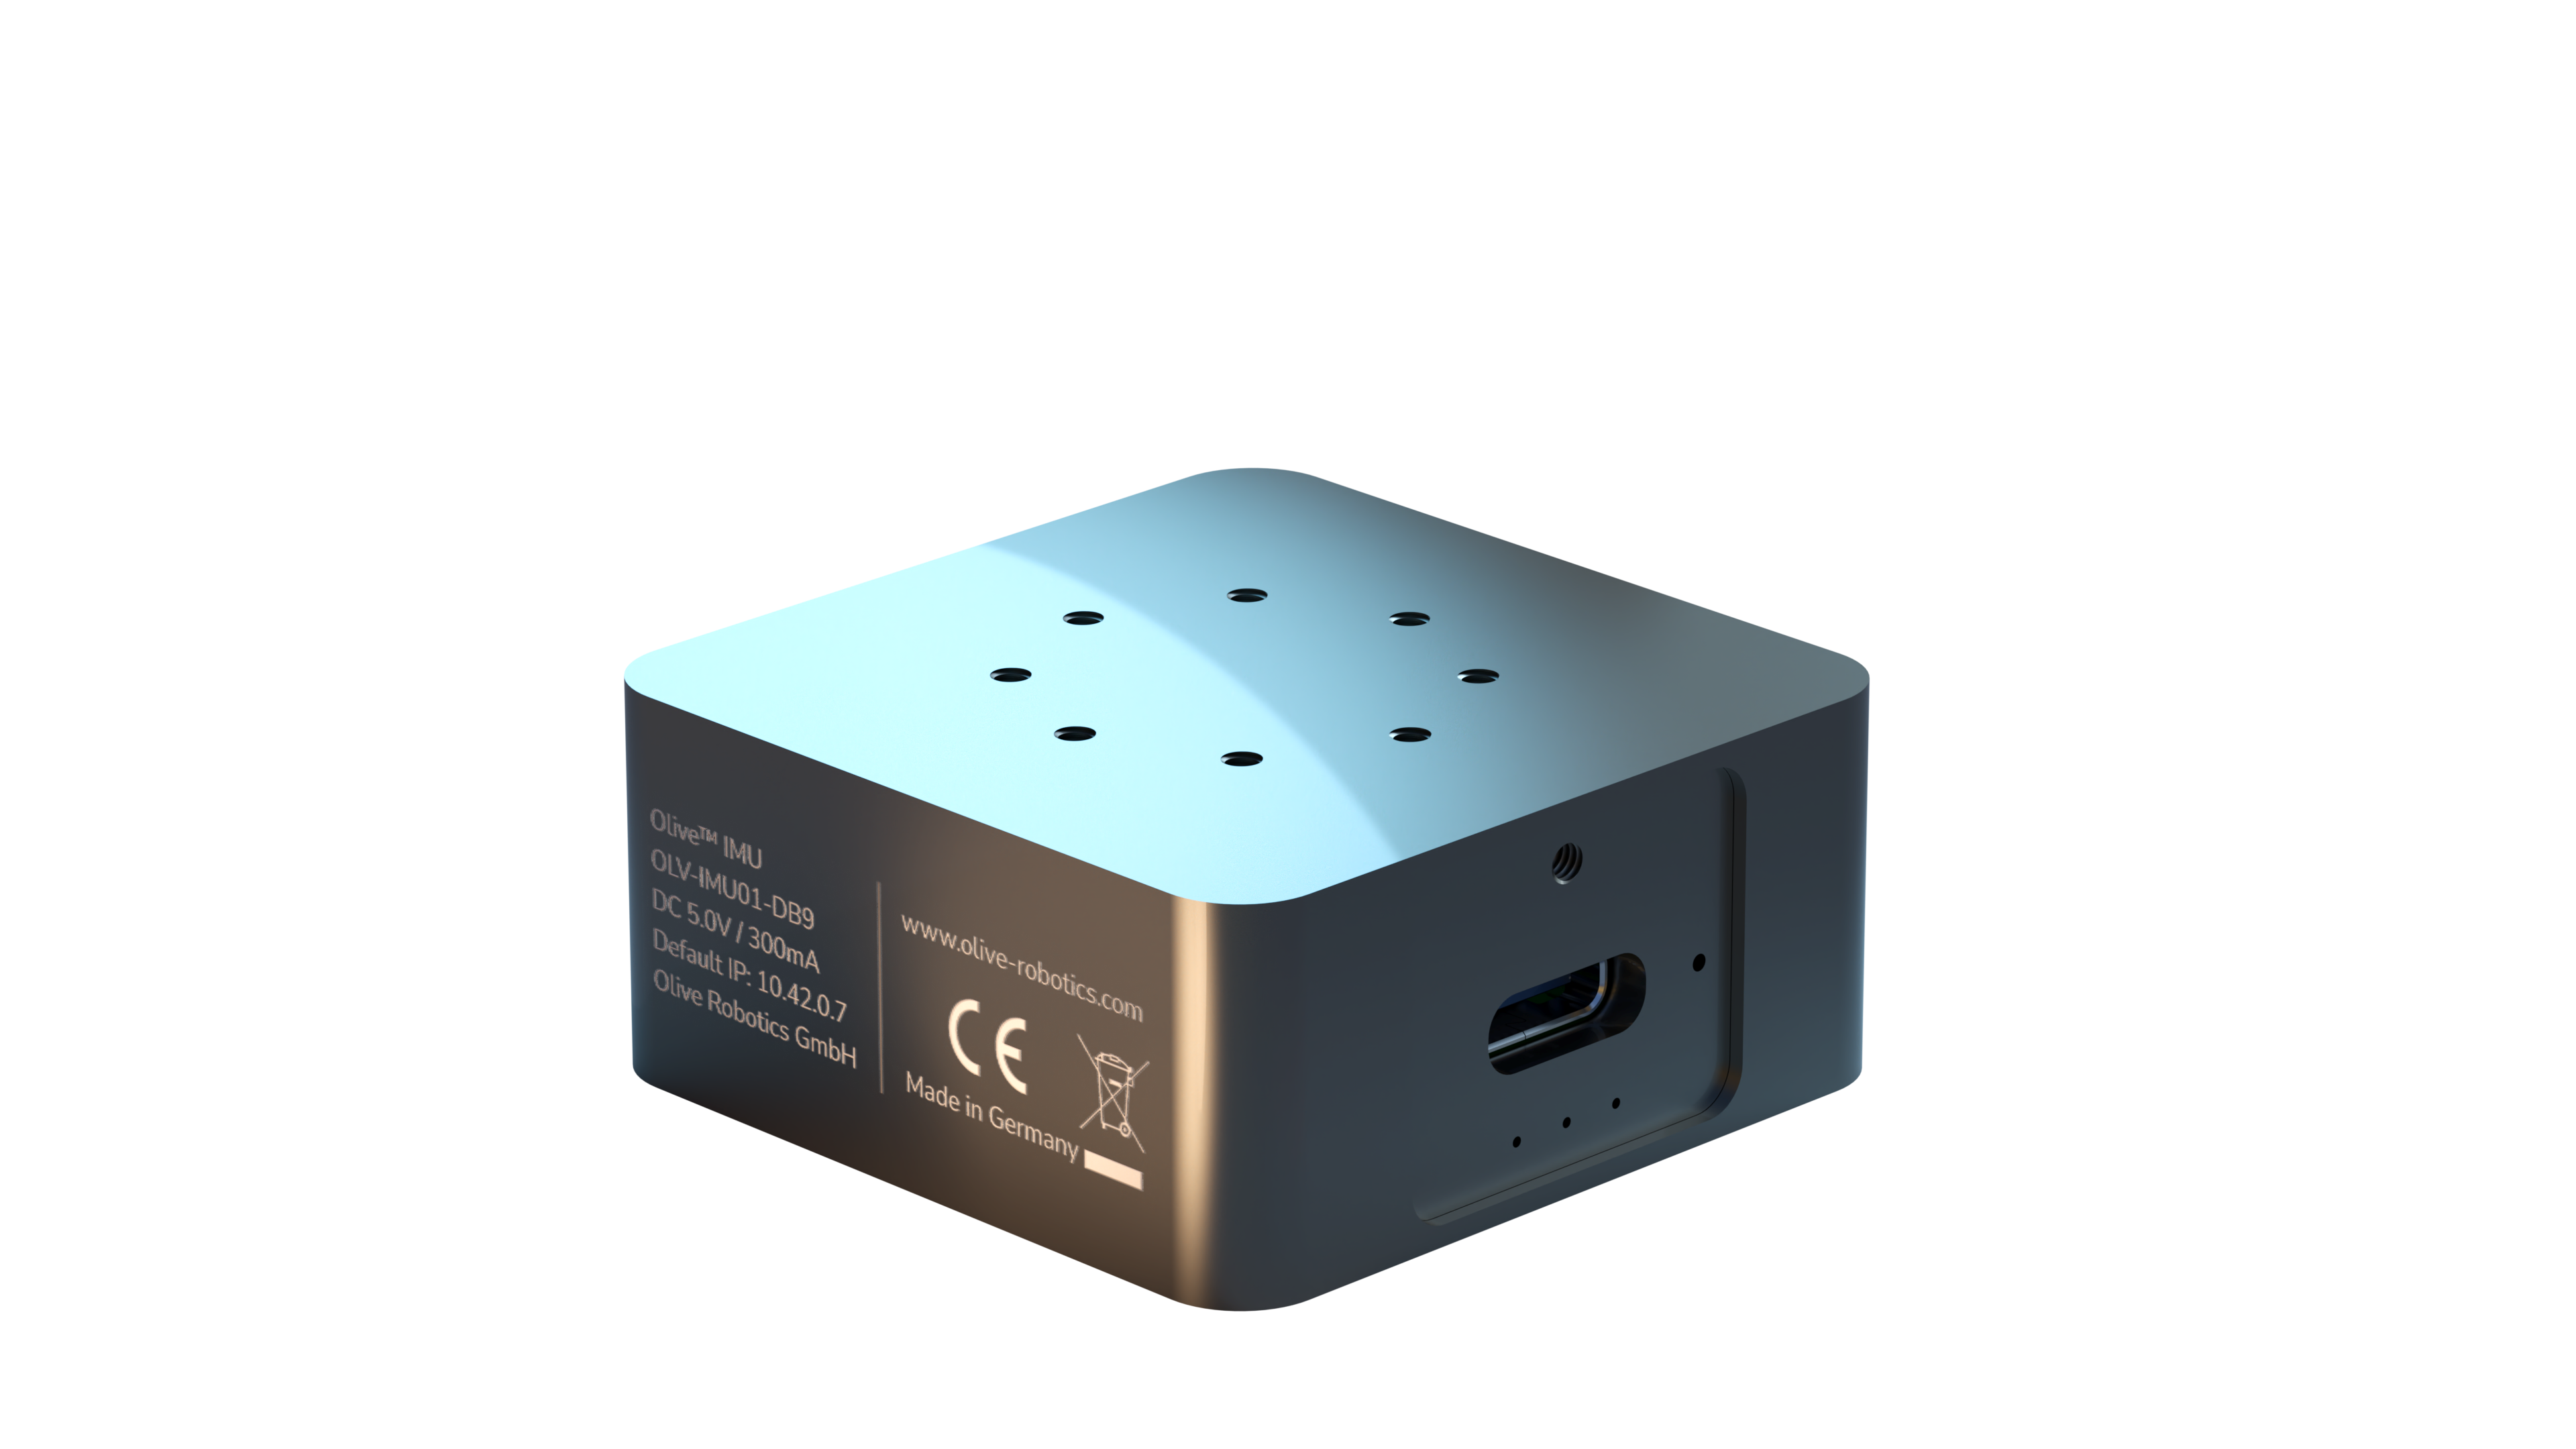
\includegraphics[width=0.5\textwidth]{img/olive_imu_v2.9d7e1d59.png}
    \caption[OLV-IMU01-13D]{OLV-IMU01-13D\footnotemark}
    \label{fig:olive_imu}
\end{figure}

\footnotetext{https://docs.olive-robotics.com/hardware/imu/imu.html}

\subsubsection{Project: IMU controls Turtle}
By utilizing the data provided by the IMU, you will control the turtle inside the turtlesim simulation. Before proceeding with writing the script, we need to take a closer look at how the IMU publishes its sensor data. Earlier, we ran the \texttt{ros2 topic list} command to list all the new topics the IMU created automatically to verify the connection. The most important topic for our specific task is the \texttt{/olive/imu/.../imu} topic, which is used for the communication of the IMU sensor data. As you already know, you can use the -t flag with this command to additionally print out all of the topic interface types.

{\lstconsolestyle
\begin{lstlisting}
$ ros2 topic list -t
/olive/imu/x1690895648100/imu [sensor_msgs/msg/Imu]
(...)    
\end{lstlisting}
}

\noindent
The interface used to communicate IMU data is called \texttt{sensor\_msgs/msg/Imu}. We previously used the \texttt{ros2 interface show} command to understand how ROS2 interfaces are defined. Since we want to use the IMU's data, we have to find out how this data is communicated.
{\lstconsolestyle
\begin{lstlisting}
$ ros2 interface show sensor_msgs/msg/Imu
# This is a message to hold data from an IMU (Inertial Measurement Unit)
#
# Accelerations should be in m/s^2 (not in g's), and rotational velocity should be in rad/sec
#
# If the covariance of the measurement is known, it should be filled in (if all you know is the
# variance of each measurement, e.g. from the datasheet, just put those along the diagonal)
# A covariance matrix of all zeros will be interpreted as "covariance unknown", and to use the
# data a covariance will have to be assumed or gotten from some other source
#
# If you have no estimate for one of the data elements (e.g. your IMU doesn't produce an
# orientation estimate), please set element 0 of the associated covariance matrix to -1
# If you are interpreting this message, please check for a value of -1 in the first element of each
# covariance matrix, and disregard the associated estimate.

std_msgs/Header header
	builtin_interfaces/Time stamp
		int32 sec
		uint32 nanosec
	string frame_id

geometry_msgs/Quaternion orientation
	float64 x 0
	float64 y 0
	float64 z 0
	float64 w 1
float64[9] orientation_covariance # Row major about x, y, z axes

geometry_msgs/Vector3 angular_velocity
	float64 x
	float64 y
	float64 z
float64[9] angular_velocity_covariance # Row major about x, y, z axes

geometry_msgs/Vector3 linear_acceleration
	float64 x
	float64 y
	float64 z
float64[9] linear_acceleration_covariance # Row major x, y z
\end{lstlisting}
}

\noindent
To control the turtle, we must determine which data from the IMU we want to utilize for this task. The most suitable data for this objective is the IMU's orientation. However, you may notice that the IMU doesn't provide Euler angles. Instead, it communicates using quaternions. Our goal is to use the pitch and yaw angles from the IMU to set the turtle's linear and angular velocity based on these angles. To obtain these angles, we need to understand how to derive them from the quaternion orientation.

\begin{figure}[H]
    \centering
    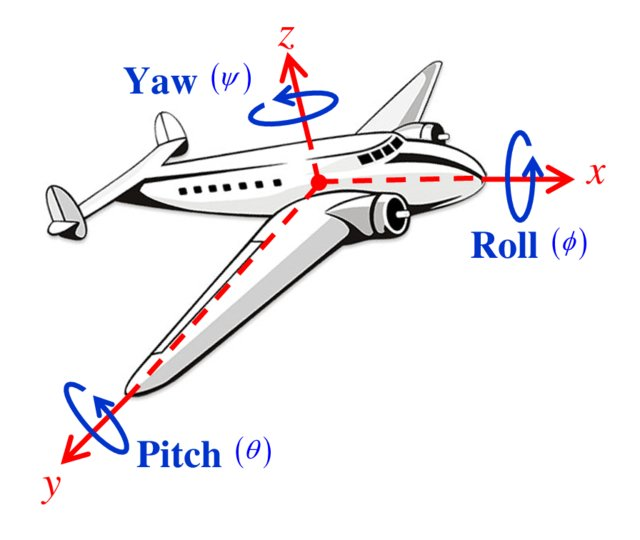
\includegraphics[width=0.5\textwidth]{img/Graphical-representation-of-Euler-angles-with-respect-to-the-reference-axis-of-the_W640.jpg}
    \caption[Euler Angles in 3D Space]{Euler Angles in 3D Space\footnotemark}
    \label{fig:euler_angles}
\end{figure}

\footnotetext{https://math.stackexchange.com/questions/4316838/are-euler-angle-figures-wrong}

\paragraph{Quaternions}~\\
Quaternions are commonly employed for calculating rotations in three-dimensional space. Unlike Euler angles, which use three values (Roll/Pitch/Yaw) to represent orientation in 3D, quaternions use four values (x, y, z, w). One of their primary advantages is that they eliminate Gimbal lock, a mathematical issue that occurs when Euler angles are used to represent 3D orientation. Gimbal lock results in the loss of a degree of freedom in three-dimensional space under specific rotation conditions.
3Blue1Brown offers an excellent video series that can help you understand quaternions\footnote{https://www.youtube.com/watch?v=zjMuIxRvygQ}. It's highly recommended to watch the first video in this series to gain a basic understanding of the topic. Generally, there is a ros2 library that is used for the rotations of quaternions called \texttt{tf2}. However, the \texttt{tf2} library, commonly used for quaternion rotations in ROS2, doesn't typically include a built-in function for converting quaternions to Euler angles. While other libraries like \texttt{tf} offer methods that could perform this conversion for us, we've chosen to implement this function ourselves for the sake of learning. To provide you with some assistance, we will supply the necessary equations required for this task. These are the mathematical expressions for the conversion\footnote{https://en.wikipedia.org/wiki/Conversion\_between\_quaternions\_and\_Euler\_angles}:

\begin{equation}
\begin{aligned}
\text{Roll (}\phi\text{)} &= atan2(2(q_w q_x + q_y q_z), 1 - 2(q_x^2 + q_y^2)) \\
\text{Pitch (}\theta\text{)} &= \arcsin(2(q_w q_y - q_z q_x)) \\
\text{Yaw (}\psi\text{)} &= atan2(2(q_w q_z + q_x q_y), 1 - 2(q_y^2 + q_z^2))
\end{aligned}
\end{equation}


\paragraph{Olive Embedded Web-based GUI}~\\
Before we proceed with writing the script, let's check out the Olive Embedded Web-based GUI. This user-friendly interface serves as a platform for configuring, controlling, and testing the modular robotic building blocks provided by Olive Robotics. By default, every time a module is connected to your PC, it is assigned the default network IP address of \texttt{10.42.0.7}. You can access the device's Web GUI by entering its IP address into your browser's search bar. It also provides an option to change this IP address, which can be helpful when connecting multiple devices to your PC simultaneously. However, for now, our focus is on utilizing its debug GUI. This feature allows us to visualize real-time orientation in Euler angles from the IMU and provides a 3D view of this data.

\paragraph{exercise}~\\
\begin{enumerate}
    \item[$\bullet$] Utilize the debug GUI to get a feeling of how the Euler angles change, dependent on the orientation of the IMU. Rotate the IMU with your hand and observe how this rotation influences the roll, pitch, and yaw angles.
\end{enumerate}

\paragraph{Project}~\\
We now have all the foundational knowledge required to implement our turtlesim IMU script. For this project, you have been given instructions to provide support, but unlike the first chapter, you'll need to handle the heavy lifting yourself. If you encounter difficulties, feel free to refer back to the previous chapter and review the specific topics you need.
\begin{enumerate}
    \item[$\bullet$] Navigate to the package directory (src) of your workspace and create a package named \texttt{olive\_imu} using the \texttt{ament\_python} build tool.

    \item[$\bullet$] Create a new Python script with the name \texttt{imu\_turtle} in the script folder of your package

    \item[$\bullet$] In your script, initialize a node that subscribes to the IMU data topic. Create an instance called \texttt{orientation} of a quaternion class within your node. In the callback function of your node, set this \texttt{orientation} object to the quaternion content of your IMU message. \textit{Hint: The quaternion message type is part of geometry\_msgs.msg}

    \item[$\bullet$] Inside your node, declare a function that takes a quaternion as input and returns the equivalent Euler angles (roll, pitch, yaw).

    \item[$\bullet$] In addition to your subscriber, create a publisher for the \texttt{/turtle/cmd\_vel} topic. Consider which Euler angles are most suitable for controlling the angular and linear velocity. If you are unsure, please refer to the Web GUI. To obtain the angles, call your new quaternion to the Euler function. Before publishing a message, ensure that you initialize a message of the correct message type and set its linear and angular velocity to the angles.

    \item[$\bullet$] Declare all the nessecary ROS2 dependencies in the package.xml of your package.

    \item[$\bullet$] Add an entry point inside your setup.py file for your script

    \item[$\bullet$] Build your package and run both the turtlesim simulator and your script to make sure it is working.

    \item[+] \textit{Create a launch file for both your turtlesim\_imu script and turtlesim\_node.} 

    \item[+] \textit{Add a parameter to adjust the speed of your turtle.}

    \item[+] \textit{Add a parameter for the name of the IMU's topic}
\end{enumerate}


\subsection{Olive Servo}
The Olive Servo\footnote{https://docs.olive-robotics.com/hardware/servo/servo.html} is used as an actuator for our robotic problems. By using its properties of rotation, we allow our systems to move in space. The module we are using in this course has three different operational modes that can be used for various problems.
\begin{enumerate}
    \item \textbf{Pulse Width Modulation} (PWM) control is a technique used to regulate the power supplied to electrical devices, such as actuators. It adjusts the duty cycle of the input signal, controlling the amount of power provided to the actuator.
    \item \textbf{Position Control} is used to maintain or adjust the position of an actuator. The controller computes the difference between the desired and actual positions and adjusts the actuator accordingly.
    \item \textbf{Velocity Control} is used to maintain or adjust the velocity of an actuator. The controller computes the difference between the desired and actual velocities and adjusts the actuator accordingly.
\end{enumerate}

\noindent
In this course, we make use of the position control that allows us to set the desired position of the servo. To achieve this, a PID controller is used to minimize the position error, adjusting the control signal to change the actuator's position.

\paragraph{PID}~\\
We are now going to discuss how the PID\footnote{https://www.elprocus.com/the-working-of-a-pid-controller/} controller is used for our purpose of setting a goal position. This section is just a summary of how PID works and not a control theory crash course. We won't discuss things like modelling the system.

\begin{figure}[H]
    \centering
    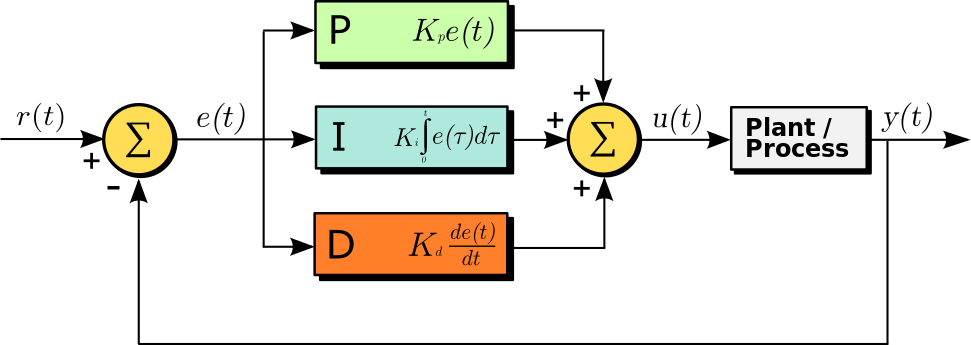
\includegraphics[width=0.5\textwidth]{img/PID_en.png}
    \caption[PID Feedback Loop]{PID Feedback Loop\footnotemark}
    \label{fig:PID}
\end{figure}

\footnotetext{https://upload.wikimedia.org/wikipedia/commons/4/43/PID\_en.svg}

\noindent
A closed-loop system, like a PID controller, includes a feedback control system. This system calculates an error signal by subtracting our current position value from our goal position. An encoder inside the servo generates the signal of its current position. We use this error signal to calculate our P, I and D values. The sum of these values is then used as a signal for the plant/process to adjust the current value. If the constants of each part are used correctly, this loop leads to the error reaching zero. Other goals that we want to achieve by setting our parameters are to reduce the time for the system to settle in and to reduce the overshoot of the system.\\

\newpage
\noindent
Following, the three parts of the PID controller will be explained. 

\begin{enumerate}
    \item[$\bullet$]\textbf{Proportional controller} (P-controller) gives an output that is proportional to current error e(t). By using a P-controller, the error is multiplied by a constant, leading to a signal proportional to the error. This controller requires biasing or manual reset when used alone. This is because it never reaches the steady-state condition. 
    \begin{equation}
        P_{out} = k_p * e(t)
    \end{equation}
    \item[$\bullet$] Due to the limitation of the P-controller, since there always exists an offset between the process variable and setpoint, an \textbf{integral controller} (I-controller) is needed. This controller provides necessary action to eliminate the steady-state error.  It integrates the error over a period of time until the error value reaches zero. It holds the value to the final control device at which the error becomes zero.
    \begin{equation}
        I_{out} = k_i \int_{0}^{t} e(\tau) d\tau   
    \end{equation}

    \item[$\bullet$]The I-controller can’t predict the future behaviour of error. So, it usually reacts once the setpoint is changed. The \textbf{derivative controller} (D-controller) overcomes this problem by anticipating the future behaviour of the error. Its output depends on the rate of change of error with respect to time, multiplied by the derivative constant. This component of our controller helps in reducing overshoot and dampening oscillations.
    \begin{equation}
        D_{out} = k_d \frac{de(t)}{dt}
    \end{equation}
\end{enumerate}
Before we test how each constant affects the movement of our servo, we have to set it up to work properly.

\paragraph{Setting up the Servo}~\\
Setting up the servo is a little bit more complicated compared to the IMU.
\begin{figure}[H]
    \centering
    \includegraphics[width=0.5\textwidth]{img/olive_servo_v2.472abedd.png}
    \caption[Olive Servo Module]{Olive Servo Module\footnotemark}
    \label{fig:Servo}
\end{figure}

\footnotetext{https://docs.olive-robotics.com/hardware/servo/servo.html}

\noindent
As shown in figure \ref{fig:Servo}, the servo module features two slots for cables. The slot with the arrow pointing towards it serves as the input, while the other slot with the arrow pointing away is designed for connecting more modules to your robot. For our current setup, we only need to use the input slot.\\
Since the output power from a laptop is insufficient to drive a servo, you'll need an additional power supply. Connect the power supply to the lightning slot on the power module of the kit and the data cable (from the PC) to the arrow slot on the module. This combination provides the necessary signal to operate the servo. Link the output of the power module to the input of the servo.\\
To verify that you've set it up correctly, you can execute the \texttt{ros2 topic list} command. Please keep in mind that it may take a moment for the system to initialize.

{\lstconsolestyle
\begin{lstlisting}
$ ros2 topic list
/olive/servo/pan/goal/position
/olive/servo/pan/joint
/olive/servo/pan/joint/diagnostics
/olive/servo/pan/led
/olive/servo/pan/status
/olive/servo/pan/switch
/olive/servo/pan/temperature
/parameter_events
/rosout
\end{lstlisting}
}


\paragraph{Utilizing the Servo}~\\
After connecting the servo, open the RQt Service Caller. Before using the servo, we need to call a service called \texttt{/olive/servo/servo\_name/setTorqueEnable}. This service was implemented as a safety feature. You can also disable the torque by calling the\\
\texttt{/olive/servo/servo\_name/setTorqueDisable }service.\\
As you may have already noticed, there is a new topic with the name \texttt{/olive/servo/pan/goal/position}. This topic is used to communicate the desired goal position to the PID controller. By publishing a message to this topic, we instruct our servo to move to the desired position.\\
When you use the \texttt{ros2 param list} command, you'll notice that the parameter values for \texttt{Kp}, \texttt{Ki}, and \texttt{Kd} appear under a node called \texttt{/olive\_servo\_pan\_dcm\_srv}. By setting these parameters, you can adjust the influence of each controller (P, I, D).\\
For the following exercises, you can use the script \ref{pid_testing_code} to alternate the goal position of a servo between \texttt{0.0} and \texttt{$\pi / 2$}.
\begin{enumerate}
    \item[$\bullet$]Begin by configuring the PID controller with the following settings: \texttt{Kp = 1.0}, \texttt{Ki = 0.0}, and \texttt{Kd = 0.0}. Observe the system's remaining error and its overshoot.
    \item[$\bullet$] Now, increase the \texttt{Kp} value. What differences do you notice when assigning new goal positions? Raise the Kp value until the servo reaches the desired speed.
    \item[$\bullet$] Introduce a \texttt{Ki} value, starting with \texttt{0.01} and observe its impact on your system. Once there is no remaining error, you can skip to the \texttt{Kd} parameter.
    \item[$\bullet$] With your current settings, you may notice an overshoot occurring. To reduce this issue, introduce the derivative (D) part to the controller. Set your \texttt{Kd} value to \texttt{1.0} and check whether this resolves the problem. Raise the value until the overshoot is eliminated.
\end{enumerate}
For the upcoming section, there's no need to adjust the parameters. These exercises were designed to enhance your comprehension of how PID controllers operate, with a focus on how each parameter impacts the controller.


\paragraph{Project: Control Servo}~\\
Currently, you have all the information you need to write a script for controlling the servo. For this project, our objective is to set position goals to move the servo in a sinusoidal motion.

\begin{enumerate}
    \item[$\bullet$] Create a new package named \texttt{olive\_servo} using the \texttt{ament\_python} build tool for this task.
    
    \item[$\bullet$] Create a script that generates a new node. This node should call the service to enable the servo.

     \item[$\bullet$] It should also publish a goal message to the goal position topic of the servo. To achieve a sinusoidal signal, you can introduce a variable that increments by a small amount every time the callback function is called. This variable can then be used as input for your sine function, and the result can be published. You can begin by selecting a publishing rate of \texttt{0.01}.
     
     \item[$\bullet$] As with the previous projects, ensure that you include all the necessary dependencies in your package and define an entry point.

     \item[$\bullet$] Test your script by running it using the \texttt{ros2 run} command.

     \item[+] \textit{Include a parameter to control the publishing frequency and observe how the system responds to different frequencies.}

     \item[+] \textit{ Call the service to disable the torque of your motor as soon as you want to close your script.}
\end{enumerate}

\subsubsection{Use 2 Servos}
Our next objective is to control two servos simultaneously. To achieve this, we need to connect two modules at the same time.

\paragraph{Network configuration}~\\
Since every module is initialized by default with the network IP address of \texttt{10.42.0.7}, we need to change them so that they are not the same. To do this, start by connecting one servo module and accessing the web interface. In the web interface, use the function to set the IP address of the lower motor to \texttt{10.42.0.8} and the upper motor to \texttt{10.42.0.9}. 

\paragraph{Project: Keyboard Control Servos}~\\
In our next project, we will finally make use of the modularity aspect of the Olive Robotics parts. The objective is to use your keyboard as input to control both servos simultaneously. Your horizontal keys will move the lower servo of your robot, while the vertical keys will control the upper servo. There are several Python libraries available for getting keyboard input. In our solution, we utilized the \texttt{pygame} library to achieve this objective.

\begin{enumerate}
    \item[$\bullet$] In your \texttt{olive\_servo package}, create a new script named \texttt{keyboard\_servos.py}.

    \item[$\bullet$] Create publishers for both goal position topics and set up a timer to call the publisher callback function every \texttt{0.01} seconds. 

    \item[$\bullet$] In your callback function, create messages based on the keyboard inputs to set the desired goals for both the upper and lower servos. Ensure to add upper and lower bounds to the published goals to prevent damaging the servos.

    \item[$\bullet$] Set an entry point for your script and test it.
    
    \item[+] \textit{Call a service to enable the torque when initializing the node and a service to disable it when the node stops spinning.} 

    \item[+] \textit{Add a parameter to adjust the speed of the servos.} 
\end{enumerate}


\paragraph{Control Olive Servos with IMU}~\\
We are now adding a third module to create a new project. Before proceeding with writing the script, set the IP address of the IMU to \texttt{10.42.0.20}. Refer to the Olive docs at \footnote{https://www.olive-robotics.com/olive-docs} and follow the \texttt{Software $>$ Olix-OS $>$ Network Configuration} guide to set up a network bridge. This step is necessary to connect several modules simultaneously to your computer. Since we need to connect one servo and the IMU to the PC, this step is important. We are going to use the orientation of the IMU to control the orientation of both motors.
\begin{enumerate}
    \item[$\bullet$] Inside your \texttt{olive\_servo package}, create a new script with the name \texttt{imu\_control\_robot.py}.

    \item[$\bullet$] Your script should contain a node with publishers for the goal positions of your motors and a subscriber for the IMU topic.

    \item[$\bullet$] Think about which Euler angles are suitable to control each servo and use these angles to publish the goal positions to each servo. You can recycle the code from previous projects to make your life a little easier. Make sure to once again add upper and lower bounds to the goal positions for protection.

    \item[$\bullet$] Add all the new dependencies to your package and create an entry point.

    \item[$\bullet$] Execute your script by using the \texttt{ros2 run} command.
    
\end{enumerate}

 
\subsection{Olive Camera}
We've reached a significant milestone for our robotic system in terms of the mobility of our robot. However, we still need to address the issue of displaying the camera's data on the screen. In this course, we're using the \texttt{OLV-CAM01-S} (figure \ref{fig:Camera_Module}) camera module, which connects to the computer via a USB C cable.

\begin{figure}[H]
    \centering
    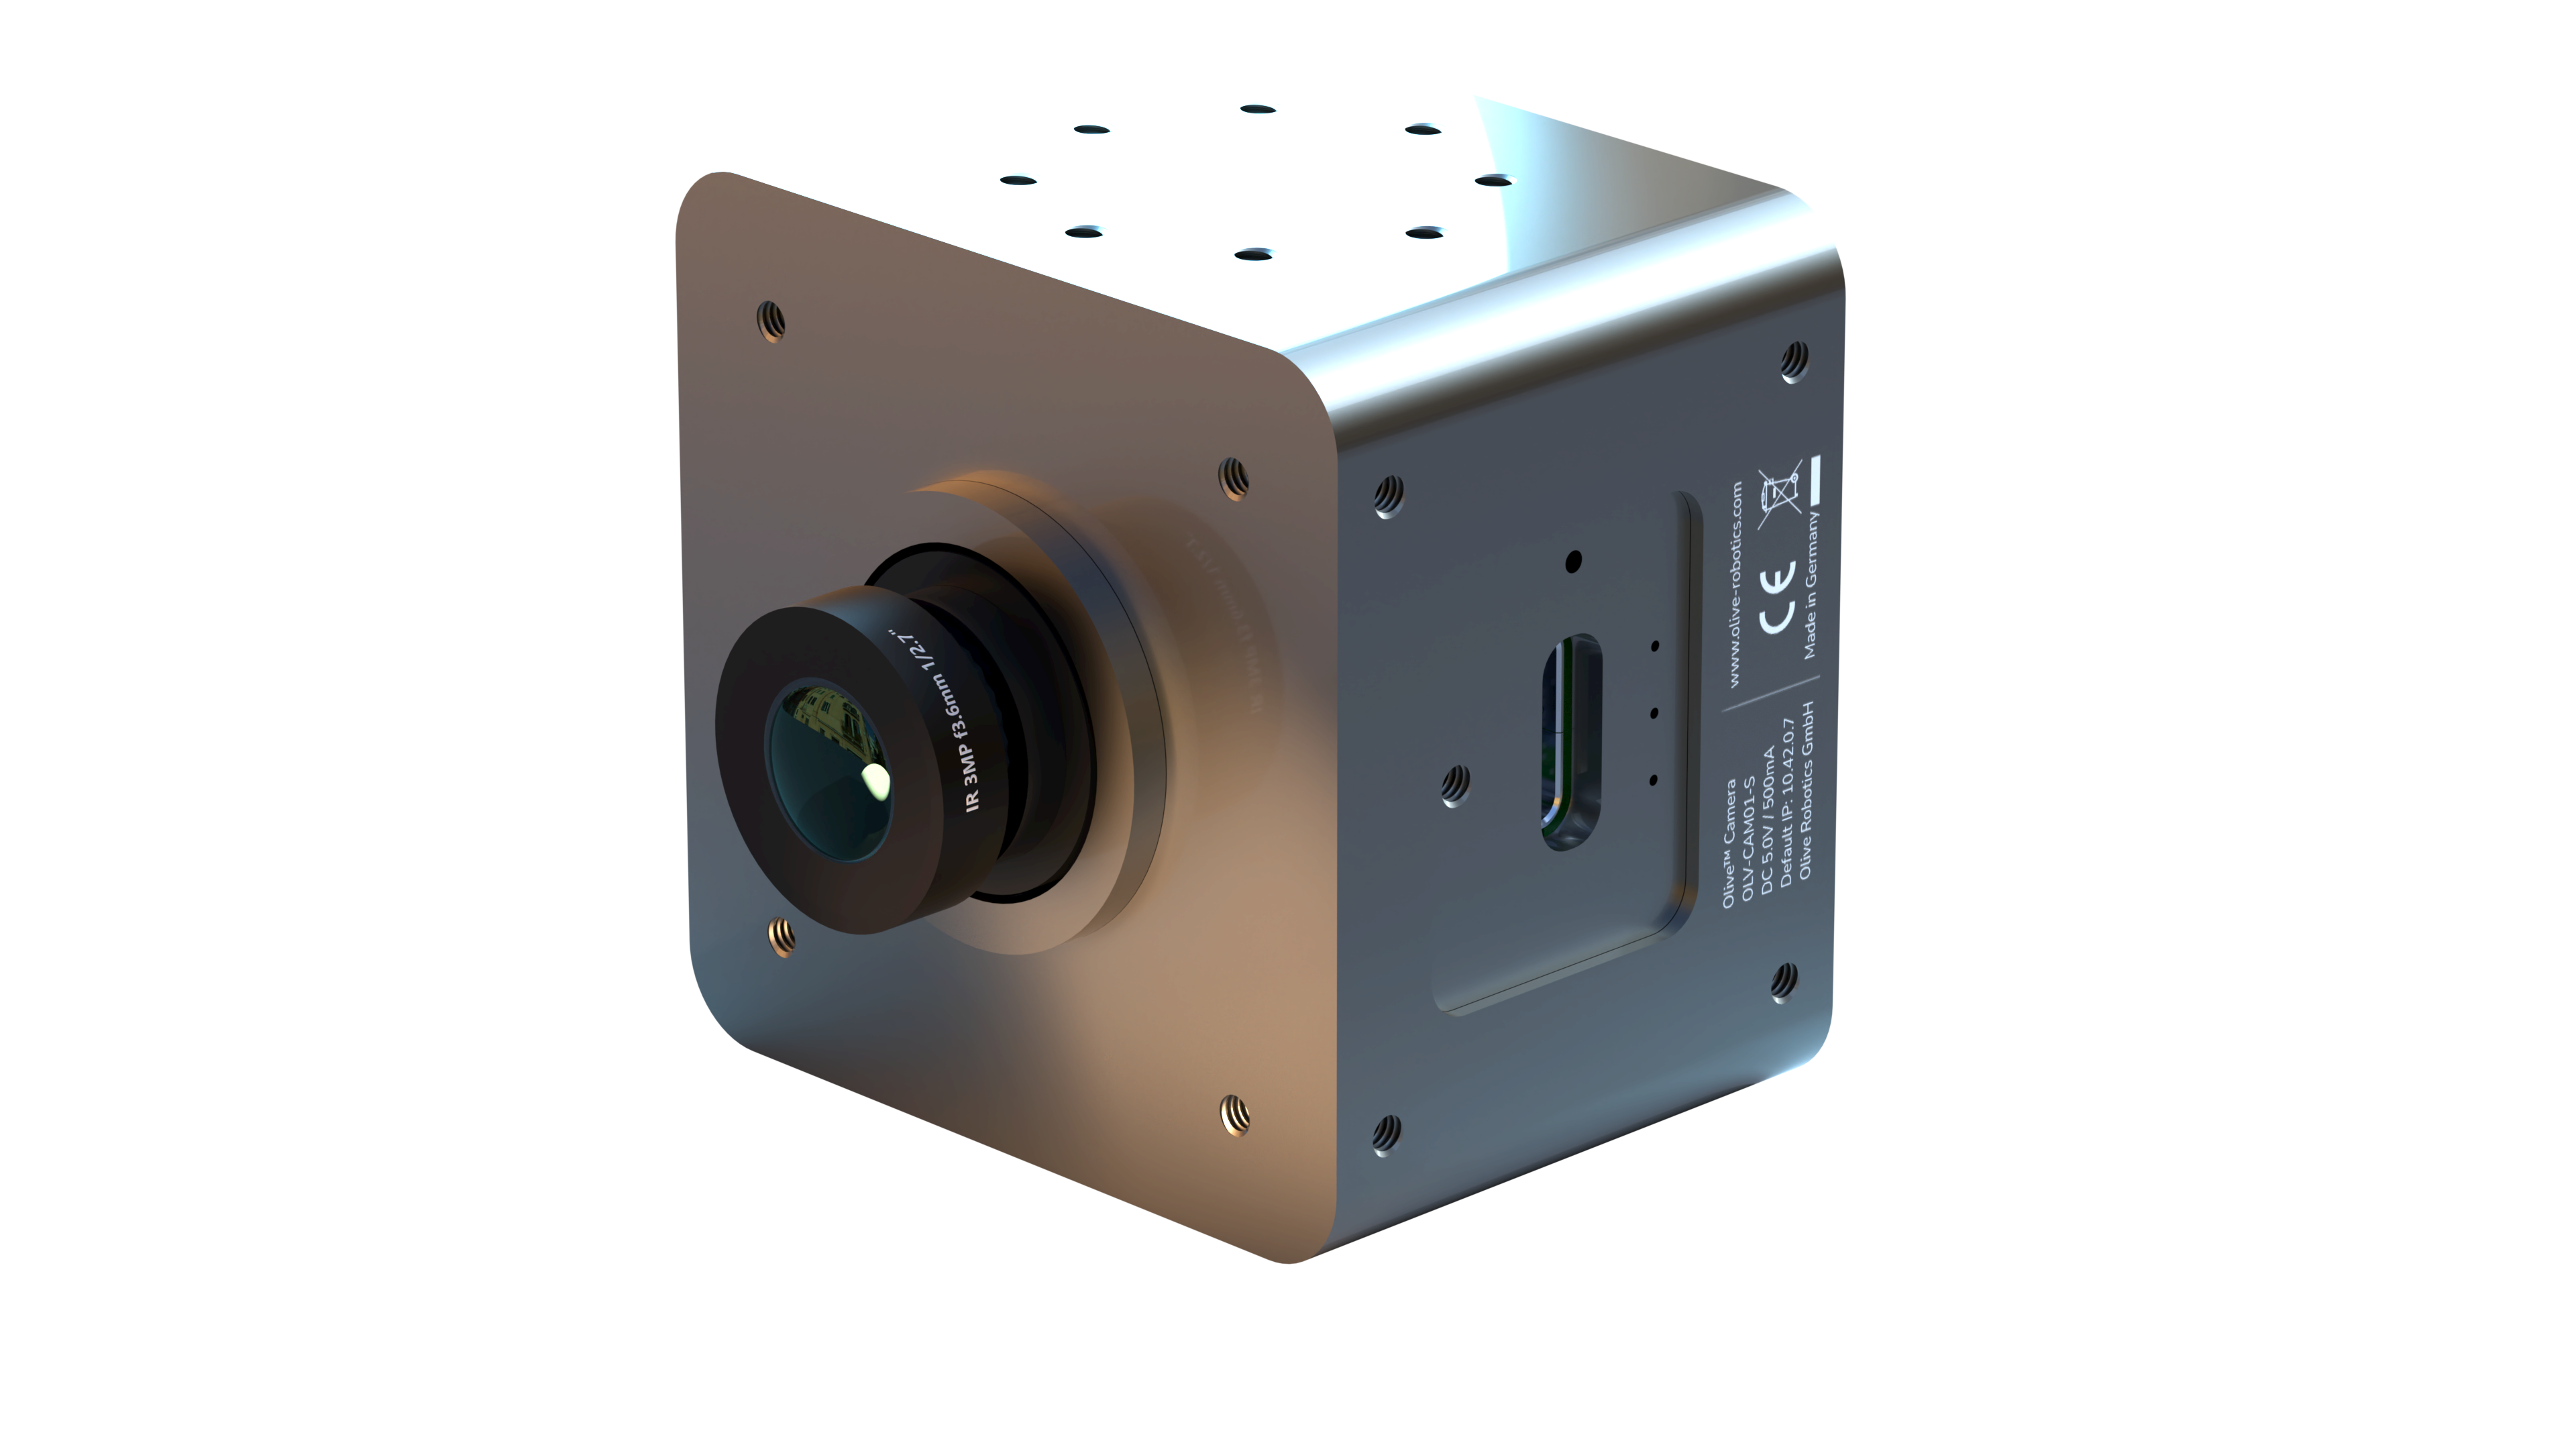
\includegraphics[width=0.5\textwidth]{img/olive-ai-camera-v2.20a7b87c.png}
    \caption[Olive Camera Module]{Olive Camera Module\footnotemark}
    \label{fig:Camera_Module}
\end{figure}

\footnotetext{https://docs.olive-robotics.com/assets/olive-ai-camera-v2.20a7b87c.png}

\noindent
Once you've connected the module, ensure that you set the camera's IP address to \texttt{10.42.0.10} and add it to the network bridge. After successfully connecting the camera, you'll notice several new topics become available. To list them along with their message types, use the \texttt{ros2 topic list -t} command.
{\lstconsolestyle
\begin{lstlisting}
$ ros2 topic list -t
/olive/camera/eye/image/camera_info [sensor_msgs/msg/CameraInfo]
/olive/camera/eye/image/compressed [sensor_msgs/msg/CompressedImage]
/olive/camera/eye/imu [sensor_msgs/msg/Imu]
/olive/camera/eye/led [std_msgs/msg/Bool]
/olive/camera/eye/magnetometer [sensor_msgs/msg/MagneticField]
/olive/camera/eye/status [diagnostic_msgs/msg/DiagnosticStatus]
/olive/camera/eye/switch [std_msgs/msg/Bool]
/olive/camera/eye/temperature [sensor_msgs/msg/Temperature]
/parameter_events [rcl_interfaces/msg/ParameterEvent]
/rosout [rcl_interfaces/msg/Log]
\end{lstlisting}
}
\noindent
The topic you're interested in, \texttt{/olive/camera/camera\_name/image/compressed}, uses the \texttt{sensor\_msgs/msg/CompressedImage} interface for communication. To understand the structure of this message type, you can use the \texttt{ros2 interface show} command, which provides detailed information about the message's structure and fields.
{\lstconsolestyle
\begin{lstlisting}
$ ros2 interface show sensor_msgs/msg/CompressedImage 
# This message contains a compressed image.

std_msgs/Header header # Header timestamp should be acquisition time of image
	builtin_interfaces/Time stamp
		int32 sec
		uint32 nanosec
	string frame_id
                             # Header frame_id should be optical frame of camera
                             # origin of frame should be optical center of cameara
                             # +x should point to the right in the image
                             # +y should point down in the image
                             # +z should point into to plane of the image

string format                # Specifies the format of the data
                             #   Acceptable values:
                             #     jpeg, png, tiff

uint8[] data                 # Compressed image buffer
\end{lstlisting}
}

\noindent
The image messages from the camera contain crucial information, such as the acquisition time, a frame ID in the header, and the image format (e.g., jpeg, png, or tiff). The essential part of these messages is the image data itself, which is represented as an 8-bit integer array, allowing values in the range of 0 to 255. To get a closer look at the structure of a message from the camera, you can examine an example message using the \texttt{ros2 topic echo} command.

{\lstconsolestyle
\begin{lstlisting}
header:
  stamp:
    sec: 1671711155
    nanosec: 577715941
  frame_id: olive
format: jpeg
data:
- 255
- 216
- 255
(...)
\end{lstlisting}
}

\noindent
To visualize the image data, we can use a program to display it on our screen. Before we create our own script for this task, we'll explore the ROS 2 solution using RQt. In RQt, go to \texttt{Plugins $>$ Visualization $>$ Image View}. In the upper left field, select the camera data topic, and you should be able to see an image displayed on your screen.\\

\noindent
Our next objective is to write our own script for displaying this image data. However, before we do that, there are still some topics we need to discuss to achieve this.


\paragraph{OpenCV}\protect\footnote{\label{fn:open_cv}http://opencv.org}~\\
To display our camera data, we'll use OpenCV, which stands for Open Source Computer Vision Library. OpenCV is an open-source library that includes hundreds of computer vision algorithms. In Python, we can access OpenCV through the cv2 module. Specifically, we'll use the \texttt{cv2.imshow(window\_name, image)} method to display the image data from our camera module on our screen.\\

\paragraph{CVBridge}\protect\footnote{\label{fn:cv_bridge}https://index.ros.org/p/cv\_bridge/\#iron}~\\
However, a challenge we encounter is that ROS 2 communicates using its own message types. Therefore, we need a tool that acts as a bridge between ROS 2 and OpenCV to convert our ROS 2 messages. One such library is called cv\_bridge. This library provides access to the CvBridge class, which contains functions like \texttt{compressed\_imgmsg\_to\_cv2(msg)} that are capable of converting ROS 2 images to OpenCV format.\\


\paragraph{QoS}\protect\footnote{\label{fn:qos}https://docs.ros.org/en/humble/Concepts/Intermediate/About-Quality-of-Service-Settings.html}~\\
Another important aspect we have to keep in mind is that we set a specific QoS profile for our subscribers. This section is a summary of the official ROS 2 docs. If you are interested in further understanding this topic, visit the website of the ROS2 docs \textsuperscript{\ref{fn:qos}}. ROS 2 offers a wide variety of Quality of Service (QoS) policies that allow you to tune communication between nodes. The base QoS profile currently includes settings for the following policies:

\begin{enumerate}
    \item[$\bullet$] \textbf{History:}\\
    \textit{Keep last:} only store up to N samples, configurable via the queue depth option.\\
    \textit{Keep all:} store all samples, subject to the configured resource limits of the underlying middleware

    \item[$\bullet$] \textbf{Depth:} \\
    \textit{Queue size:} only honoured if the “history” policy was set to “keep last”

    \item[$\bullet$] \textbf{Reliability:}\\
    \textit{Best effort:} attempt to deliver samples but may lose them if the network is not robust
    \textit{Reliable:} guarantee that samples are delivered may retry multiple times

    \item[$\bullet$] \textbf{Durability:}\\
    \textit{Transient local:} the publisher becomes responsible for persisting samples for “late-joining” subscriptions\\
    \textit{Volatile:} no attempt is made to persist samples

    \item[$\bullet$] \textbf{Deadline:}\\
    \textit{Duration:} the expected maximum amount of time between subsequent messages being published to a topic

    \item[$\bullet$] \textbf{Lifespan:}\\
    \textit{Duration:} the maximum amount of time between the publishing and the reception of a message without the message being considered stale or expired (expired messages are silently dropped and are effectively never received)
    
    \item[$\bullet$] \textbf{Liveliness:}\\
    \textit{Automatic:} the system will consider all of the node’s publishers to be alive for another “lease duration” when any one of its publishers has published a message\\
    \textit{Manual by topic:} The system will consider the publisher to be alive for another “lease duration” if it manually asserts that it is still alive (via a call to the publisher API)
    
    \item[$\bullet$] \textbf{Lease Duration:}\\
    \textit{Duration:} the maximum period of time a publisher has to indicate that it is alive before the system considers it to have lost liveliness (losing liveliness could be an indication of a failure)
\end{enumerate}

\noindent
Profiles allow developers to focus on their applications without worrying about every QoS setting possible. A QoS profile defines a set of policies that are expected to go well together for a particular use case.\\

\noindent
QoS profiles may be configured for publishers and subscriptions independently. A connection between a publisher and a subscription is only made if the pair has compatible QoS profiles.\\

\noindent
QoS profile compatibility is determined based on a “Request vs Offered” model. Subscriptions request a QoS profile that defines the “minimum quality” that it is willing to accept, and publishers offer a QoS profile that defines the “maximum quality” that it is able to provide. Connections are only made if every policy of the requested QoS profile is not more stringent than that of the offered QoS profile. Multiple subscriptions can be connected to a single publisher simultaneously, even if their requested QoS profiles are different. The compatibility between a publisher and a subscription is unaffected by the presence of other publishers and subscriptions.\\

\noindent
To know how we have to set up the QoS settings of our subscribing node, we have to get the QoS settings of our publishing node. An easy way to do this is using the \texttt{-v} or \texttt{--verbose} flag for our \texttt{ros2 topic info} command. It prints detailed information like the node name, node namespace, topic type, GUID and QoS profile of the publishers and subscribers to this topic. Using this command on our camera node returns:

{\lstconsolestyle
\begin{lstlisting}
$ ros2 topic info /olive/camera/eye/image/compressed -v
(...)
QoS profile:
  Reliability: BEST_EFFORT
  History (Depth): UNKNOWN
  Durability: VOLATILE
  Lifespan: Infinite
  Deadline: Infinite
  Liveliness: AUTOMATIC
  Liveliness lease duration: Infinite
(...)
\end{lstlisting}
}

\noindent
Since our publisher node uses specific QoS settings, we need to adjust the QoS settings of our subscribing node. To determine which settings are compatible with each other, it is recommended to take a look at the source page for QoS on the ROS2 docs\textsuperscript{\ref{fn:qos}}. The ROS2 docs provide a table with different settings for publishers and subscribers that work well together. In our case, we need to configure the reliability and durability options for a proper connection. The \texttt{best\_effort} policy used by our publisher requires us to set the reliability policy of our subscriber to \texttt{best\_effort} as well. The same settings should be applied to the durability policy (\texttt{volatile}).\\

\noindent
To create a custom QoS profile in Python, we must import the QoS profile class from \texttt{rclpy.qos}. When creating a QoS profile, we provide the desired QoS policies as input. Since we want to set the reliability and durability policies, we also need to import them from \texttt{rclpy.qos}. So far, we have set the \texttt{depth} option for our subscribing nodes by specifying an integer in the QoS profile. This policy allows us to create a queue that improves our connection. We also want to apply this policy to our camera profile.\\

\noindent
The following lines of code demonstrate how to create this profile in a Python script.

\begin{minted}{python}
from rclpy.qos import QoSProfile, QoSDurabilityPolicy, QoSReliabilityPolicy

qos_profile = QoSProfile(
            depth=10,
            durability=QoSDurabilityPolicy.VOLATILE,
            reliability=QoSReliabilityPolicy.BEST_EFFORT)
\end{minted}

\paragraph{Project: Display Camera}~\\
Our final objective is to create a Python script that displays the data from your camera module on your screen.

\begin{enumerate}
    \item[$\bullet$] Create a new package with the name \texttt{olive\_camera} and inside of it a new script called \texttt{display\_camera.py}.

    \item[$\bullet$] Create a new node that subscribes to the compressed image topic of your camera module. Remember to create a custom QoS profile for your subscriber. 

    \item[$\bullet$] Initialize a CvBridge object and use it to transform your ROS2 message to a CV2 object. Utilize the \texttt{imshow} command to create your display window. Don't forget to import all the necessary modules.

    \item[$\bullet$] Add all the necessary dependencies and add an entry point for your script. Test your script using \texttt{ros2 run}.

    \item[$\bullet$] Run the script for controlling the robot with your IMU and display the camera content using your new script.

    \item[+] \textit{Create a launch file for \texttt{imu\_control\_robot} and \texttt{display\_camera}}.
        
\end{enumerate}

\paragraph{Course Ending}~\\
Congratulations, you have successfully completed this course. If you are interested in furthering your ROS2 knowledge and delving into more complex topics, feel free to visit the official ROS2 docs\footnote{https://docs.ros.org/en/humble/index.html}.

\subsection{Use Object Tracking}
This section is intended to be a suggestion for the future expansion of this course.
%-get the coordinate of the detected object
%-calculate the error dx, dy
%-goal position = goal position +dx , dy

\subsection{Use Gesture Control}
This section is intended to be a suggestion for the future expansion of this course.

%-optional
\newpage
\section{Appendix}

\subsection{ROS2 Commands}

\begin{table}[H]
    \centering
    \begin{tabular}{|p{6cm}|p{8cm}|}
        \hline
        \textbf{ROS2 Command} & \textbf{Explanation} \\
        \hline
        \texttt{ros2 run} & Run a ROS2 node from a specific package. \\
        \hline
        \texttt{ros2 node list} & List all active nodes in the ROS2 system. \\
        \hline
        \texttt{ros2 node info} & Provides information about a specific ROS2 node. \\
        \hline
        \texttt{rqt} & Launches the ROS graphical user interface tool. \\
        \hline
        \texttt{ros2 topic list} & Lists all available topics in the ROS2 system. \\
        \hline
        \texttt{ros2 topic info} & Provides information about a specific ROS2 topic. \\
        \hline
        \texttt{ros2 interface show} & Displays the message type definition for a given ROS2 interface. \\
        \hline
        \texttt{ros2 topic echo} & Displays messages being published on a specific topic. \\
        \hline
        \texttt{ros2 topic pub} & Publishes messages to a specific topic. \\
        \hline
        \texttt{colcon build} & Builds ROS2 packages using the colcon build system. \\
        \hline
        \texttt{ros2 pkg list} & Lists available ROS2 packages. \\
        \hline
        \texttt{ros2 pkg create} & Creates a new ROS2 package. \\
        \hline
        \texttt{ros2 service list} & Lists available ROS2 services. \\
        \hline
        \texttt{ros2 service type} & Displays the service type of a specific ROS2 service. \\
        \hline
        \texttt{ros2 service call} & Calls a ROS2 service with specified request data. \\
        \hline
        \texttt{ros2 param list} & Lists available ROS2 parameters. \\
        \hline
        \texttt{ros2 param get} & Retrieves the value of a specific ROS2 parameter. \\
        \hline
        \texttt{ros2 param set} & Sets the value of a specific ROS2 parameter. \\
        \hline
        \texttt{ros2 param dump} & Dumps parameter values to a file. \\
        \hline
        \texttt{ros2 param load} & Loads parameter values from a file. \\
        \hline
        \texttt{ros2 action list} & Lists available ROS2 action interfaces. \\
        \hline
        \texttt{ros2 action info} & Displays information about a specific ROS2 action interface. \\
        \hline
        \texttt{ros2 action send\_goal} & Sends a goal to a ROS2 action server. \\
        \hline
        \texttt{ros2 launch} & Launches ROS2 launch files. \\
        \hline
    \end{tabular}
    \caption{ROS2 Commands and Explanations}
    \label{tab:ros2-commands}
\end{table}

\subsection{Linux Commands}

\begin{table}[H]
    \centering
    \begin{tabular}{|p{6cm}|p{8cm}|}
        \hline
        
        \textbf{Linux Command} & \textbf{Explanation} \\
        \hline
        
        \texttt{cd $<$dir$>$} & Change directory to dir \\
        \hline
        
        \texttt{cd ..} & Go up a directory \\
        \hline
        
        \texttt{ls} & List files \\
        \hline

        \texttt{mkdir $<$dir$>$} & make directory  $<$dir$>$\\
        \hline

        \texttt{pwd} & show current directory\\
        \hline
        
    \end{tabular}
    \caption{Linux Commands and Explanations}
    \label{tab:linux-commands}
\end{table}


\subsection{Code PID testing\label{pid_testing_code}}

\begin{minted}{python}
import math
import rclpy
from rclpy.node import Node

from std_msgs.msg import Float32
from std_srvs.srv import Trigger


class ControlServo(Node):

    def __init__(self):
        super().__init__("control_servo")
        self.service_enable_torque = self.create_client(Trigger,
        "/olive/servo/pan/setTorqueEnable")
        self.service_disable_torque = self.create_client(Trigger,
        "/olive/servo/pan/setTorqueDisable")
        while not self.service_enable_torque.wait_for_service(timeout_sec=1.0):
            self.get_logger().info("service not available")
        while not self.service_disable_torque.wait_for_service(timeout_sec=1.0):
            self.get_logger().info("service not available")
        self.request_enable_torque = Trigger.Request()
        self.request_disable_torque = Trigger.Request()
        self.topic_gp = "/olive/servo/pan/goal/position"
        self.publisher = self.create_publisher(Float32, self.topic_gp, 10)
        self.timer = self.create_timer(3.0, self.publish_goal)
        self.state = True

    def enable_torque(self):
        self.future = self.service_enable_torque.call_async(self.request_enable_torque)
        rclpy.spin_until_future_complete(self, self.future)

    def disable_torque(self):
        self.future = self.service_disable_torque.call_async(self.request_disable_torque)
        rclpy.spin_until_future_complete(self, self.future)

    def publish_goal(self):
        msg = Float32()

        if self.state == True:
            msg.data = 1.57
            self.state = False
        else:
            msg.data = 0.0
            self.state = True

        self.publisher.publish(msg)

def main():
    rclpy.init()
    cntrl_publisher = ControlServo()
    
    try:
        cntrl_publisher.enable_torque()
        rclpy.spin(cntrl_publisher)
    except KeyboardInterrupt:
        cntrl_publisher.disable_torque()
        cntrl_publisher.destroy_node()
        rclpy.shutdown()

if __name__ == "__main__":
    main()
\end{minted}





% ------------------------------------------------------------------------------
% Reference and Cited Works
% ------------------------------------------------------------------------------



% ------------------------------------------------------------------------------

\end{document}
